\documentclass[10pt,a4paper]{article}
\usepackage[utf8]{inputenc}
\usepackage[margin=0.6in]{geometry}
\usepackage{listings}
\usepackage{xcolor}
\usepackage{graphicx}
\usepackage{multicol}

% Code listing settings - compact version
\lstset{
    language=[Sharp]C,
    basicstyle=\ttfamily\scriptsize,
    keywordstyle=\color{blue}\bfseries,
    commentstyle=\color{green!50!black}\itshape,
    stringstyle=\color{red},
    numbers=left,
    numberstyle=\tiny\color{gray},
    stepnumber=1,
    numbersep=5pt,
    backgroundcolor=\color{gray!5},
    showspaces=false,
    showstringspaces=false,
    showtabs=false,
    frame=single,
    tabsize=2,
    captionpos=b,
    breaklines=true,
    breakatwhitespace=false,
    aboveskip=8pt,
    belowskip=8pt,
    xleftmargin=10pt,
    escapeinside={\%*}{*)},
    morekeywords={var, async, await, from, select, where, orderby, group, into, let, join}
}

\setlength{\parindent}{0pt}
\setlength{\parskip}{6pt}
\setlength{\columnsep}{20pt}

\begin{document}

% ======================== LAB 1 ========================
\newpage
\section*{Lab 1: Five Types of Constructor in C\#}

\textbf{Title:} Write a C\# program to demonstrate five types of constructor in C\#.

\subsection*{Theory}
Constructors are special methods that initialize objects when they are created. They have the same name as the class and no return type.

Five types of constructors:
\begin{itemize}
    \item \textbf{Default Constructor} - No parameters, initializes with default values
    \item \textbf{Parameterized Constructor} - Accepts parameters to set specific values
    \item \textbf{Copy Constructor} - Creates object by copying another object
    \item \textbf{Static Constructor} - Initializes static members, called once automatically
    \item \textbf{Private Constructor} - Prevents object creation from outside (used in Singleton pattern)
\end{itemize}

\subsection*{Code}
\begin{multicols}{2}
\begin{lstlisting}
using System;

class ConstructorDemo
{
    private int value;
    private string name;

    // 1. Default Constructor
    public ConstructorDemo()
    {
        value = 0;
        name = "Default";
        Console.WriteLine("Default Constructor: value={0}, name={1}", 
                         value, name);
    }

    // 2. Parameterized Constructor
    public ConstructorDemo(int val, string nm)
    {
        value = val;
        name = nm;
        Console.WriteLine("Parameterized Constructor: value={0}, name={1}", 
                         value, name);
    }

    // 3. Copy Constructor
    public ConstructorDemo(ConstructorDemo obj)
    {
        value = obj.value;
        name = obj.name;
        Console.WriteLine("Copy Constructor: value={0}, name={1}", 
                         value, name);
    }

    // 4. Static Constructor
    static ConstructorDemo()
    {
        Console.WriteLine("Static Constructor called");
    }
}

// 5. Private Constructor
class Singleton
{
    private static Singleton instance;

    private Singleton()
    {
        Console.WriteLine("Private Constructor called");
    }

    public static Singleton GetInstance()
    {
        if (instance == null)
            instance = new Singleton();
        return instance;
    }
}

class Program
{
    static void Main()
    {
        ConstructorDemo obj1 = new ConstructorDemo();
        ConstructorDemo obj2 = new ConstructorDemo(10, "Test");
        ConstructorDemo obj3 = new ConstructorDemo(obj2);
        Singleton s = Singleton.GetInstance();

        Console.WriteLine("\nLab No.: 1");
        Console.WriteLine("Name: Samir Paudel");
        Console.WriteLine("Roll No./Section: 114-079/D");
    }
}
\end{lstlisting}
\end{multicols}

\subsection*{Output}
\begin{figure}[h!]
    \raggedright
    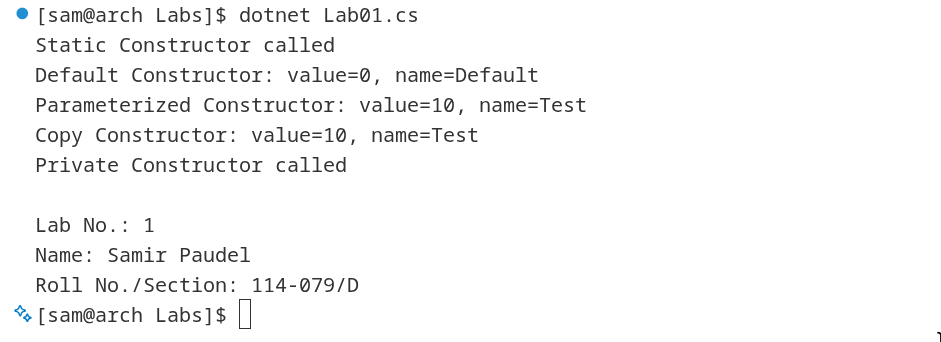
\includegraphics[width=0.4\linewidth]{lab01.png}
\end{figure}

\newpage

% ======================== LAB 2 ========================
\section*{Lab 2: Auto Property and Read-Only Property}

\subsection*{Title}
WAP in C\# to demonstrate concept of auto Property and Read-Only Property.

\subsection*{Theory}
\textbf{Auto-implemented Properties:} Provide a simplified syntax for property declaration where the compiler automatically creates a private backing field. Syntax: \texttt{public Type PropertyName \{ get; set; \}}

\textbf{Read-Only Properties:} Properties that can only be read, not modified. They have only a \texttt{get} accessor. Read-only properties can be initialized in the constructor or with an initializer.

Auto properties make code more concise and eliminate the need to explicitly declare backing fields for simple properties.

\subsection*{Code}
\begin{multicols}{2}
\begin{lstlisting}
using System;

class Person
{
    // Auto-implemented property with get and set
    public string Name { get; set; }
    
    // Auto-implemented property with default value
    public int Age { get; set; } = 0;
    
    // Read-only auto property (can only be set in constructor)
    public string Country { get; }
    
    // Read-only property with backing field
    private string _ssn;
    public string SSN 
    { 
        get { return _ssn; } 
    }
    
    // Auto property with private setter
    public string Email { get; private set; }
    
    // Constructor
    public Person(string country, string ssn)
    {
        Country = country;  // Can set read-only property in constructor
        _ssn = ssn;
    }
    
    public void SetEmail(string email)
    {
        Email = email;  // Can set via method since setter is private
    }
    
    public void DisplayInfo()
    {
        Console.WriteLine($"Name: {Name}");
        Console.WriteLine($"Age: {Age}");
        Console.WriteLine($"Country: {Country}");
        Console.WriteLine($"SSN: {SSN}");
        Console.WriteLine($"Email: {Email}");
    }
}

class Program
{
    static void Main()
    {
        Person person = new Person("Nepal", "123-45-6789");
        
        // Setting auto properties
        person.Name = "Ram Sharma";
        person.Age = 25;
        person.SetEmail("ram@example.com");
        
        Console.WriteLine("Person Information:");
        person.DisplayInfo();
        
        // Attempting to modify read-only property will cause compile error
        // person.Country = "India";  // Error!
        // person.SSN = "987-65-4321";  // Error!
        
        Console.WriteLine("\nLab No.: 2");
        Console.WriteLine("Name: Samir Paudel");
        Console.WriteLine("Roll No./Section: 114-079/D");
    }
}
\end{lstlisting}
\end{multicols}

\subsection*{Output}
\begin{figure}[h!]
    \raggedright
    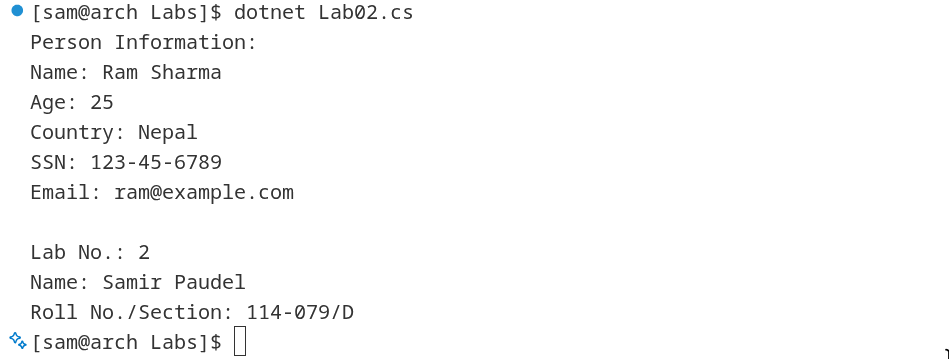
\includegraphics[width=0.7\linewidth]{lab02.png}
\end{figure}

\newpage

% ======================== LAB 3 ========================
\section*{Lab 3: Jagged Array}

\subsection*{Title}
WAP in C\# to demonstrate jagged array.

\subsection*{Theory}
A \textbf{jagged array} is an array of arrays where each element is itself an array. Unlike multidimensional arrays, the arrays in a jagged array can have different lengths.

Syntax: \texttt{type[][] arrayName = new type[rows][];}

Jagged arrays are useful when you need to store rows of data with varying numbers of columns, making them more memory-efficient than rectangular arrays for irregular data structures.

\subsection*{Code}
\begin{multicols}{2}
\begin{lstlisting}
using System;

class JaggedArrayDemo
{
    static void Main()
    {
        // Declare jagged array with 4 rows
        int[][] jaggedArray = new int[4][];
        
        // Initialize each row with different lengths
        jaggedArray[0] = new int[3] { 1, 2, 3 };
        jaggedArray[1] = new int[5] { 4, 5, 6, 7, 8 };
        jaggedArray[2] = new int[2] { 9, 10 };
        jaggedArray[3] = new int[4] { 11, 12, 13, 14 };
        
        Console.WriteLine("Jagged Array Elements:");
        Console.WriteLine("======================");
        
        // Display jagged array
        for (int i = 0; i < jaggedArray.Length; i++)
        {
            Console.Write($"Row {i}: ");
            for (int j = 0; j < jaggedArray[i].Length; j++)
            {
                Console.Write(jaggedArray[i][j] + " ");
            }
            Console.WriteLine();
        }
        
        // Another example with user input simulation
        Console.WriteLine("\nStudent Marks (Different subjects per student):");
        Console.WriteLine("===============================================");
        
        int[][] studentMarks = new int[3][];
        studentMarks[0] = new int[] { 85, 90, 78, 92 };      // 4 subjects
        studentMarks[1] = new int[] { 88, 76 };              // 2 subjects
        studentMarks[2] = new int[] { 95, 89, 91 };          // 3 subjects
        
        for (int i = 0; i < studentMarks.Length; i++)
        {
            Console.Write($"Student {i + 1} marks: ");
            double sum = 0;
            for (int j = 0; j < studentMarks[i].Length; j++)
            {
                Console.Write(studentMarks[i][j] + " ");
                sum += studentMarks[i][j];
            }
            double average = sum / studentMarks[i].Length;
            Console.WriteLine($"(Average: {average:F2})");
        }
        
        Console.WriteLine("\nLab No.: 3");
        Console.WriteLine("Name: Samir Paudel");
        Console.WriteLine("Roll No./Section: 114-079/D");
    }
}
\end{lstlisting}
\end{multicols}

\subsection*{Output}
\begin{figure}[h!]
    \raggedright
    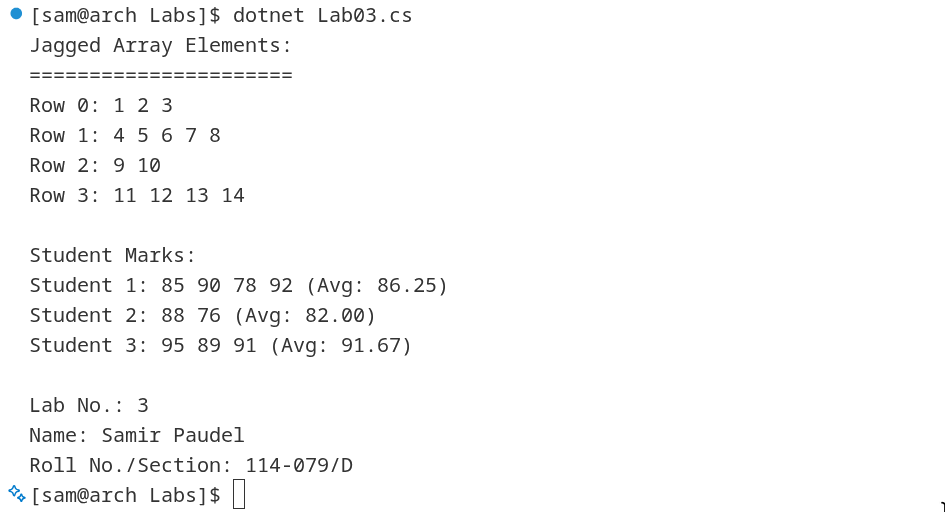
\includegraphics[width=0.5\linewidth]{lab03.png}
\end{figure}

\newpage

% ======================== LAB 4 ========================
\section*{Lab 4: Indexer in C\#}

\subsection*{Title}
WAP to demonstrate Indexer in C\#:\\
a) When index is of int type\\
b) When index is of other than int type.

\subsection*{Theory}
\textbf{Indexers} allow objects to be indexed like arrays. They enable instances of a class to be accessed using array-like syntax.

Syntax: \texttt{type this[type index] \{ get \{\} set \{\} \}}

Indexers can be of different types:
\begin{itemize}
    \item \textbf{Integer indexer} - Uses int type for index (most common)
    \item \textbf{String indexer} - Uses string type for index (like dictionary)
    \item \textbf{Other types} - Can use any type as index parameter
\end{itemize}

\subsection*{Code}
\begin{multicols}{2}
\begin{lstlisting}
using System;

// Example 1: Integer Indexer
class StudentMarks
{
    private int[] marks = new int[5];
    
    // Integer indexer
    public int this[int index]
    {
        get 
        { 
            if (index >= 0 && index < marks.Length)
                return marks[index];
            else
                throw new IndexOutOfRangeException("Index out of range");
        }
        set 
        { 
            if (index >= 0 && index < marks.Length)
                marks[index] = value;
            else
                throw new IndexOutOfRangeException("Index out of range");
        }
    }
    
    public int Length
    {
        get { return marks.Length; }
    }
}

// Example 2: String Indexer
class PhoneBook
{
    private string[] names = new string[10];
    private string[] phones = new string[10];
    private int count = 0;
    
    // String indexer
    public string this[string name]
    {
        get
        {
            for (int i = 0; i < count; i++)
            {
                if (names[i] == name)
                    return phones[i];
            }
            return "Not Found";
        }
        set
        {
            for (int i = 0; i < count; i++)
            {
                if (names[i] == name)
                {
                    phones[i] = value;
                    return;
                }
            }
            // Add new entry
            if (count < names.Length)
            {
                names[count] = name;
                phones[count] = value;
                count++;
            }
        }
    }
    
    public void Display()
    {
        Console.WriteLine("\nPhone Book Entries:");
        for (int i = 0; i < count; i++)
        {
            Console.WriteLine($"{names[i]}: {phones[i]}");
        }
    }
}

class Program
{
    static void Main()
    {
        // Integer Indexer Demo
        Console.WriteLine("=== Integer Indexer Demo ===");
        StudentMarks student = new StudentMarks();
        
        student[0] = 85;
        student[1] = 90;
        student[2] = 78;
        student[3] = 92;
        student[4] = 88;
        
        Console.WriteLine("Student Marks:");
        for (int i = 0; i < student.Length; i++)
        {
            Console.WriteLine($"Subject {i + 1}: {student[i]}");
        }
        
        // String Indexer Demo
        Console.WriteLine("\n=== String Indexer Demo ===");
        PhoneBook phoneBook = new PhoneBook();
        
        phoneBook["Ram"] = "9841234567";
        phoneBook["Sita"] = "9847654321";
        phoneBook["Hari"] = "9851112222";
        phoneBook["Gita"] = "9863334444";
        
        phoneBook.Display();
        
        Console.WriteLine($"\nRam's phone: {phoneBook["Ram"]}");
        Console.WriteLine($"Sita's phone: {phoneBook["Sita"]}");
        Console.WriteLine($"Unknown: {phoneBook["Unknown"]}");
        
        Console.WriteLine("\nLab No.: 4");
        Console.WriteLine("Name: Samir Paudel");
        Console.WriteLine("Roll No./Section: 114-079/D");
    }
}
\end{lstlisting}
\end{multicols}

\subsection*{Output}
\begin{figure}[h!]
    \raggedright
    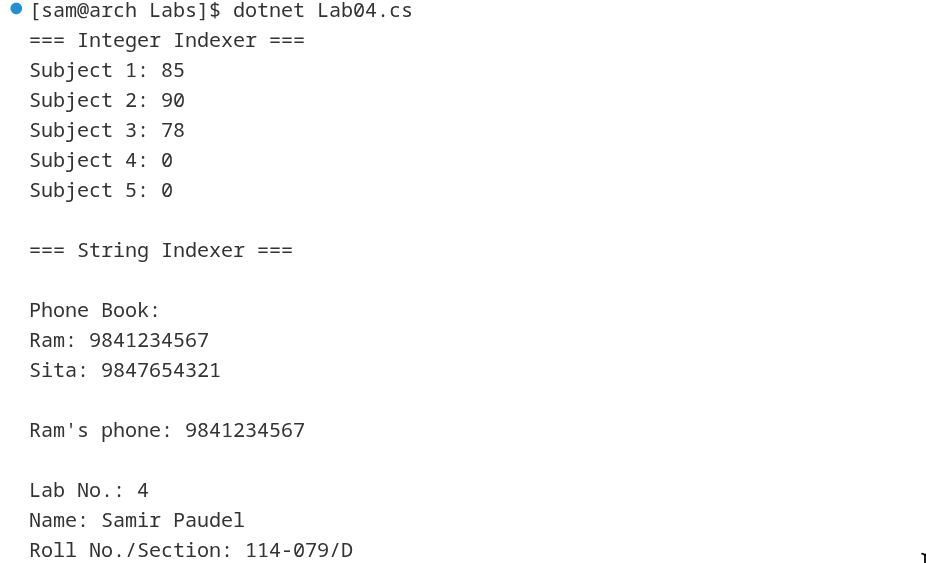
\includegraphics[width=0.7\linewidth]{lab04.png}
\end{figure}

\newpage

% ======================== LAB 5 ========================
\section*{Lab 5: Base Keyword in C\#}

\subsection*{Title}
WAP to demonstrate:\\
a) The use of base keyword to access base class fields\\
b) The use of base keyword to call base class methods\\
c) The use of base keyword to call base class constructor

\subsection*{Theory}
The \textbf{base} keyword is used to access members of the base class from within a derived class.

Three main uses of base keyword:
\begin{itemize}
    \item \textbf{Access base class fields} - When derived class has a field with the same name
    \item \textbf{Call base class methods} - To invoke an overridden method from the base class
    \item \textbf{Call base class constructor} - To invoke a specific base class constructor
\end{itemize}

The base keyword is essential for extending base class functionality while maintaining access to original implementations.

\subsection*{Code}
\begin{multicols}{2}
\begin{lstlisting}
using System;

// Base class
class Vehicle
{
    protected string brand = "Generic Brand";
    protected int speed = 0;
    
    public Vehicle()
    {
        Console.WriteLine("Vehicle: Default constructor called");
    }
    
    public Vehicle(string brand, int speed)
    {
        this.brand = brand;
        this.speed = speed;
        Console.WriteLine($"Vehicle: Parameterized constructor called");
    }
    
    public virtual void ShowInfo()
    {
        Console.WriteLine($"Brand: {brand}, Speed: {speed} km/h");
    }
    
    public void StartEngine()
    {
        Console.WriteLine($"{brand}: Engine started");
    }
}

// Derived class
class Car : Vehicle
{
    private string brand = "Car Brand";  // Hides base class field
    private int numberOfDoors;
    
    // a) Using base keyword to call base class constructor
    public Car() : base()
    {
        numberOfDoors = 4;
        Console.WriteLine("Car: Default constructor called");
    }
    
    public Car(string brand, int speed, int doors) : base(brand, speed)
    {
        numberOfDoors = doors;
        Console.WriteLine("Car: Parameterized constructor called");
    }
    
    // b) Using base keyword to call base class method
    public override void ShowInfo()
    {
        Console.WriteLine("--- Car Information ---");
        base.ShowInfo();  // Call base class ShowInfo()
        Console.WriteLine($"Number of Doors: {numberOfDoors}");
    }
    
    // c) Using base keyword to access base class field
    public void DisplayBrands()
    {
        Console.WriteLine($"Base class brand: {base.brand}");
        Console.WriteLine($"Derived class brand: {this.brand}");
    }
    
    public void StartCarEngine()
    {
        base.StartEngine();  // Call base class method
        Console.WriteLine("Car-specific systems initialized");
    }
}

class Program
{
    static void Main()
    {
        Console.WriteLine("=== Creating Car with default constructor ===");
        Car car1 = new Car();
        Console.WriteLine();
        
        Console.WriteLine("=== Creating Car with parameterized constructor ===");
        Car car2 = new Car("Toyota", 180, 4);
        Console.WriteLine();
        
        Console.WriteLine("=== Demonstrating base keyword uses ===\n");
        
        // a) Accessing base class fields using base keyword
        Console.WriteLine("1. Accessing base class fields:");
        car2.DisplayBrands();
        Console.WriteLine();
        
        // b) Calling base class method using base keyword
        Console.WriteLine("2. Calling base class method:");
        car2.ShowInfo();
        Console.WriteLine();
        
        // c) Using base keyword in constructor (already demonstrated above)
        Console.WriteLine("3. Starting engine (calls base class method):");
        car2.StartCarEngine();
        
        Console.WriteLine("\nLab No.: 5");
        Console.WriteLine("Name: Samir Paudel");
        Console.WriteLine("Roll No./Section: 114-079/D");
    }
}
\end{lstlisting}
\end{multicols}

\subsection*{Output}
\begin{figure}[h!]
    \raggedright
    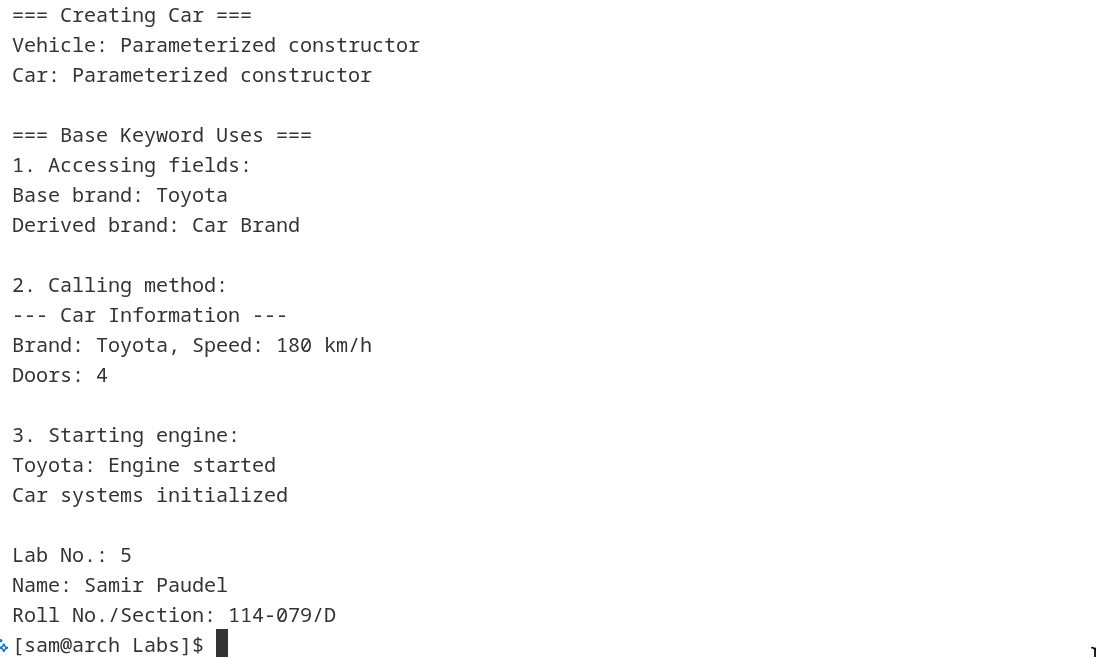
\includegraphics[width=0.7\linewidth]{lab05.png}
\end{figure}

\newpage

% ======================== LAB 6 ========================
\section*{Lab 6: Method Overriding and Dynamic Polymorphism}

\subsection*{Title}
Program to show:\\
a) method overriding and method hiding/shadowing in C\#\\
b) dynamic polymorphism using method overriding.

\subsection*{Theory}
\textbf{Method Overriding:} Allows a derived class to provide a specific implementation of a method that is already defined in its base class. Uses \texttt{virtual} and \texttt{override} keywords.

\textbf{Method Hiding/Shadowing:} Uses the \texttt{new} keyword to hide a base class method with the same name in a derived class.

\textbf{Dynamic Polymorphism:} Also known as runtime polymorphism, achieved through method overriding. The method to be called is determined at runtime based on the actual object type.

Key differences:
\begin{itemize}
    \item Override maintains polymorphic behavior
    \item New breaks polymorphism and hides the base method
\end{itemize}

\subsection*{Code}
\begin{multicols}{2}
\begin{lstlisting}
using System;

// Base class
class Shape
{
    protected string name;
    
    public Shape(string name)
    {
        this.name = name;
    }
    
    // Virtual method for overriding
    public virtual void Draw()
    {
        Console.WriteLine($"Drawing a {name}");
    }
    
    // Method for hiding demonstration
    public void ShowInfo()
    {
        Console.WriteLine($"This is a {name}");
    }
    
    public virtual double CalculateArea()
    {
        return 0;
    }
}

// Derived class 1: Circle
class Circle : Shape
{
    private double radius;
    
    public Circle(double radius) : base("Circle")
    {
        this.radius = radius;
    }
    
    // Method Overriding using override keyword
    public override void Draw()
    {
        Console.WriteLine($"Drawing a circle with radius {radius}");
    }
    
    public override double CalculateArea()
    {
        return Math.PI * radius * radius;
    }
    
    // Method Hiding using new keyword
    public new void ShowInfo()
    {
        Console.WriteLine($"This is a Circle with radius {radius}");
    }
}

// Derived class 2: Rectangle
class Rectangle : Shape
{
    private double length, width;
    
    public Rectangle(double length, double width) : base("Rectangle")
    {
        this.length = length;
        this.width = width;
    }
    
    // Method Overriding
    public override void Draw()
    {
        Console.WriteLine($"Drawing rectangle: {length} x {width}");
    }
    
    public override double CalculateArea()
    {
        return length * width;
    }
    
    // Method Hiding
    public new void ShowInfo()
    {
        Console.WriteLine($"This is a Rectangle: {length} x {width}");
    }
}

class Program
{
    static void Main()
    {
        Console.WriteLine("=== Method Overriding vs Method Hiding ===\n");
        
        Circle circle = new Circle(5.0);
        Rectangle rectangle = new Rectangle(4.0, 6.0);
        
        // Direct calls
        Console.WriteLine("--- Direct Method Calls ---");
        circle.Draw();
        circle.ShowInfo();
        Console.WriteLine($"Circle Area: {circle.CalculateArea():F2}\n");
        
        rectangle.Draw();
        rectangle.ShowInfo();
        Console.WriteLine($"Rectangle Area: {rectangle.CalculateArea():F2}\n");
        
        // Dynamic Polymorphism (Runtime Polymorphism)
        Console.WriteLine("--- Dynamic Polymorphism ---");
        Shape shape1 = new Circle(7.0);
        Shape shape2 = new Rectangle(5.0, 8.0);
        
        // Overridden methods show polymorphic behavior
        Console.WriteLine("Using base class reference:");
        shape1.Draw();  // Calls Circle's Draw()
        Console.WriteLine($"Area: {shape1.CalculateArea():F2}");
        
        shape2.Draw();  // Calls Rectangle's Draw()
        Console.WriteLine($"Area: {shape2.CalculateArea():F2}");
        
        Console.WriteLine();
        
        // Hidden methods do NOT show polymorphic behavior
        Console.WriteLine("Hidden method (new keyword) behavior:");
        shape1.ShowInfo();  // Calls Shape's ShowInfo(), not Circle's
        shape2.ShowInfo();  // Calls Shape's ShowInfo(), not Rectangle's
        
        Console.WriteLine();
        
        // Array of shapes demonstrating dynamic polymorphism
        Console.WriteLine("--- Array of Shapes (Dynamic Polymorphism) ---");
        Shape[] shapes = new Shape[3];
        shapes[0] = new Circle(3.0);
        shapes[1] = new Rectangle(4.0, 5.0);
        shapes[2] = new Circle(6.0);
        
        foreach (Shape s in shapes)
        {
            s.Draw();
            Console.WriteLine($"Area: {s.CalculateArea():F2}\n");
        }
        
        Console.WriteLine("Lab No.: 6");
        Console.WriteLine("Name: Samir Paudel");
        Console.WriteLine("Roll No./Section: 114-079/D");
    }
}
\end{lstlisting}
\end{multicols}

\subsection*{Output}
\begin{figure}[h!]
    \raggedright
    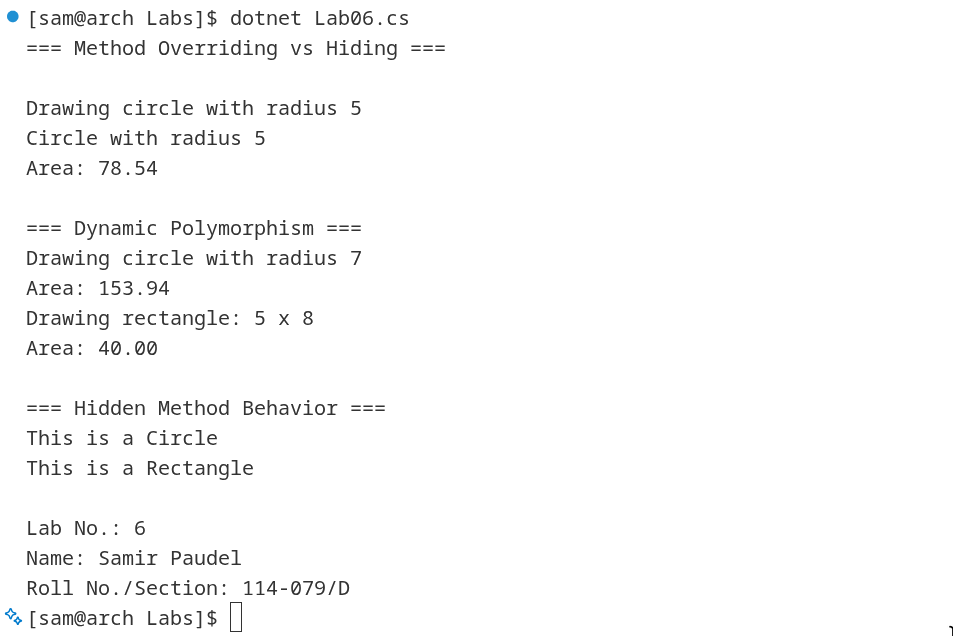
\includegraphics[width=0.7\linewidth]{lab06.png}
\end{figure}

\newpage

% ======================== LAB 7 ========================
\section*{Lab 7: Abstract Class, Interface, and Multiple Inheritance}

\subsection*{Title}
WAP to illustrate the concept of:\\
a) Abstract class\\
b) Interface\\
c) Multiple inheritance using interface in C\#

\subsection*{Theory}
\textbf{Abstract Class:} A class that cannot be instantiated and may contain both abstract and non-abstract methods. Used as a base class. Declared using \texttt{abstract} keyword.

\textbf{Interface:} A contract that defines a set of methods and properties without implementation. Classes implementing an interface must provide implementation for all its members.

\textbf{Multiple Inheritance:} C\# doesn't support multiple inheritance with classes but supports it through interfaces. A class can implement multiple interfaces.

Key differences:
\begin{itemize}
    \item Abstract class can have implementation; interface cannot (before C\# 8.0)
    \item A class can inherit only one abstract class but multiple interfaces
    \item Abstract class can have fields; interface cannot
\end{itemize}

\subsection*{Code}
\begin{multicols}{2}
\begin{lstlisting}
using System;

// a) Abstract Class
abstract class Animal
{
    protected string name;
    
    public Animal(string name)
    {
        this.name = name;
    }
    
    // Abstract method (must be implemented by derived classes)
    public abstract void MakeSound();
    
    // Non-abstract method (can be used by derived classes)
    public void Sleep()
    {
        Console.WriteLine($"{name} is sleeping...");
    }
    
    // Abstract method
    public abstract void Move();
}

// b) Interfaces
interface IFlyable
{
    void Fly();
    int MaxAltitude { get; set; }
}

interface ISwimmable
{
    void Swim();
    int MaxDepth { get; set; }
}

interface IRunnable
{
    void Run();
}

// Derived class from abstract class
class Dog : Animal, IRunnable
{
    public Dog(string name) : base(name) { }
    
    public override void MakeSound()
    {
        Console.WriteLine($"{name} says: Woof! Woof!");
    }
    
    public override void Move()
    {
        Console.WriteLine($"{name} is running on four legs");
    }
    
    public void Run()
    {
        Console.WriteLine($"{name} is running fast!");
    }
}

// c) Multiple Inheritance using Interfaces
class Duck : Animal, IFlyable, ISwimmable
{
    public int MaxAltitude { get; set; }
    public int MaxDepth { get; set; }
    
    public Duck(string name) : base(name)
    {
        MaxAltitude = 1000;
        MaxDepth = 10;
    }
    
    public override void MakeSound()
    {
        Console.WriteLine($"{name} says: Quack! Quack!");
    }
    
    public override void Move()
    {
        Console.WriteLine($"{name} can walk, fly, and swim");
    }
    
    public void Fly()
    {
        Console.WriteLine($"{name} is flying up to {MaxAltitude} meters");
    }
    
    public void Swim()
    {
        Console.WriteLine($"{name} is swimming down to {MaxDepth} meters");
    }
}

class Bird : Animal, IFlyable
{
    public int MaxAltitude { get; set; }
    
    public Bird(string name) : base(name)
    {
        MaxAltitude = 5000;
    }
    
    public override void MakeSound()
    {
        Console.WriteLine($"{name} says: Tweet! Tweet!");
    }
    
    public override void Move()
    {
        Console.WriteLine($"{name} is flying");
    }
    
    public void Fly()
    {
        Console.WriteLine($"{name} is flying at {MaxAltitude} meters altitude");
    }
}

class Program
{
    static void Main()
    {
        Console.WriteLine("=== Abstract Class Demo ===\n");
        
        Dog dog = new Dog("Buddy");
        dog.MakeSound();
        dog.Move();
        dog.Sleep();
        dog.Run();
        
        Console.WriteLine("\n=== Interface Demo ===\n");
        
        Bird bird = new Bird("Sparrow");
        bird.MakeSound();
        bird.Move();
        bird.Fly();
        bird.Sleep();
        
        Console.WriteLine("\n=== Multiple Inheritance using Interface ===\n");
        
        Duck duck = new Duck("Donald");
        duck.MakeSound();
        duck.Move();
        duck.Fly();
        duck.Swim();
        duck.Sleep();
        
        Console.WriteLine("\n=== Polymorphism with Abstract Class ===\n");
        
        Animal[] animals = { dog, bird, duck };
        foreach (Animal animal in animals)
        {
            animal.MakeSound();
            animal.Move();
            Console.WriteLine();
        }
        
        Console.WriteLine("=== Interface Reference ===\n");
        
        IFlyable[] flyingThings = { bird, duck };
        foreach (IFlyable flyer in flyingThings)
        {
            flyer.Fly();
        }
        
        Console.WriteLine("\nLab No.: 7");
        Console.WriteLine("Name: Samir Paudel");
        Console.WriteLine("Roll No./Section: 114-079/D");
    }
}
\end{lstlisting}
\end{multicols}

\subsection*{Output}
\begin{figure}[h!]
    \raggedright
    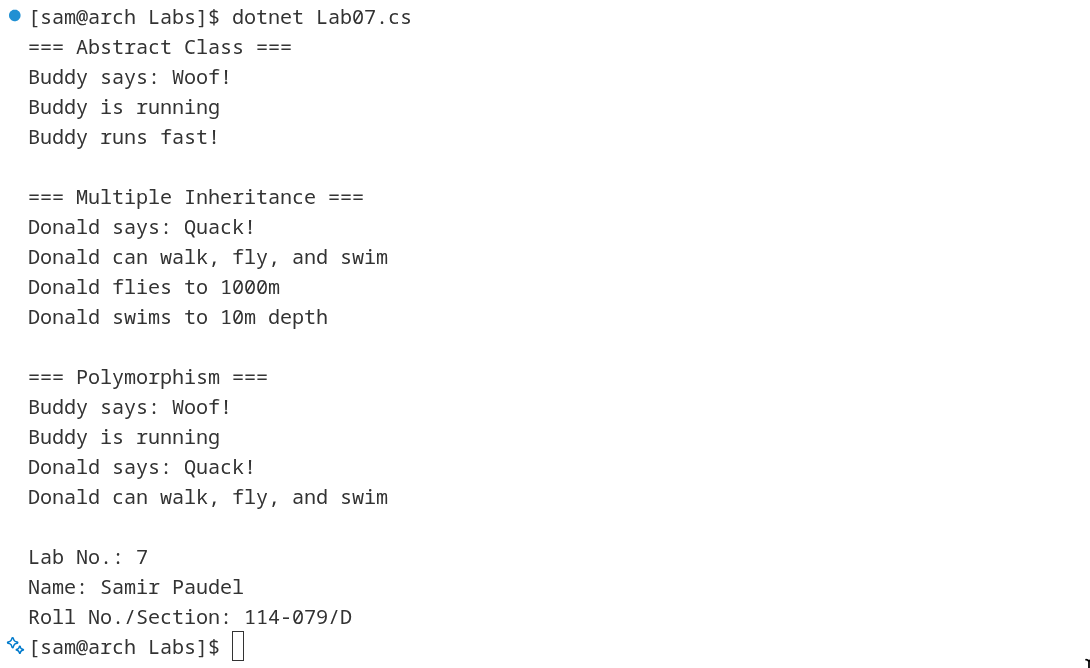
\includegraphics[width=0.7\linewidth]{lab07.png}
\end{figure}

\newpage

% ======================== LAB 8 ========================
\section*{Lab 8: Structure, Enumeration, and Partial Class}

\subsection*{Title}
WAP program that contains:\\
a) Structure (struct)\\
b) Enumeration (enum)\\
c) Partial class

\subsection*{Theory}
\textbf{Structure (struct):} A value type that can contain data members and function members. Structures are stored on the stack and are suitable for small data structures.

\textbf{Enumeration (enum):} A value type consisting of a set of named constants. Used to define a group of related integral constants.

\textbf{Partial Class:} Allows splitting the definition of a class across multiple files. All parts must use the \texttt{partial} keyword and will be combined during compilation.

Key points:
\begin{itemize}
    \item Struct is value type; class is reference type
    \item Enum provides readable names for numeric values
    \item Partial classes help organize large classes and support code generation
\end{itemize}

\subsection*{Code}
\begin{multicols}{2}
\begin{lstlisting}
using System;

// a) Structure (struct)
struct Point
{
    public int X;
    public int Y;
    
    public Point(int x, int y)
    {
        X = x;
        Y = y;
    }
    
    public void Display()
    {
        Console.WriteLine($"Point: ({X}, {Y})");
    }
    
    public double DistanceFromOrigin()
    {
        return Math.Sqrt(X * X + Y * Y);
    }
}

struct Student
{
    public int RollNo;
    public string Name;
    public double Marks;
    
    public Student(int rollNo, string name, double marks)
    {
        RollNo = rollNo;
        Name = name;
        Marks = marks;
    }
    
    public void DisplayInfo()
    {
        Console.WriteLine($"Roll No: {RollNo}");
        Console.WriteLine($"Name: {Name}");
        Console.WriteLine($"Marks: {Marks}");
        Console.WriteLine($"Grade: {GetGrade()}");
    }
    
    public string GetGrade()
    {
        if (Marks >= 90) return "A+";
        else if (Marks >= 80) return "A";
        else if (Marks >= 70) return "B+";
        else if (Marks >= 60) return "B";
        else if (Marks >= 50) return "C";
        else return "F";
    }
}

// b) Enumeration (enum)
enum Days
{
    Sunday,
    Monday,
    Tuesday,
    Wednesday,
    Thursday,
    Friday,
    Saturday
}

enum OrderStatus
{
    Pending = 1,
    Processing = 2,
    Shipped = 3,
    Delivered = 4,
    Cancelled = 5
}

enum Priority
{
    Low = 1,
    Medium = 2,
    High = 3,
    Critical = 4
}

// c) Partial Class (Part 1)
partial class Employee
{
    private int empId;
    private string name;
    private double salary;
    
    public Employee(int id, string name, double salary)
    {
        this.empId = id;
        this.name = name;
        this.salary = salary;
    }
    
    public void DisplayBasicInfo()
    {
        Console.WriteLine($"Employee ID: {empId}");
        Console.WriteLine($"Name: {name}");
        Console.WriteLine($"Salary: {salary:C}");
    }
}

// c) Partial Class (Part 2)
partial class Employee
{
    public void CalculateBonus()
    {
        double bonus = salary * 0.10;
        Console.WriteLine($"Bonus: {bonus:C}");
        Console.WriteLine($"Total: {(salary + bonus):C}");
    }
    
    public void GiveRaise(double percentage)
    {
        double raise = salary * (percentage / 100);
        salary += raise;
        Console.WriteLine($"Salary increased by {percentage}%");
        Console.WriteLine($"New Salary: {salary:C}");
    }
}

class Program
{
    static void Main()
    {
        Console.WriteLine("=== STRUCTURE Demo ===\n");
        
        Point p1 = new Point(3, 4);
        p1.Display();
        Console.WriteLine($"Distance from origin: {p1.DistanceFromOrigin():F2}");
        
        Console.WriteLine();
        
        Student student = new Student(101, "Ram Kumar", 85.5);
        student.DisplayInfo();
        
        Console.WriteLine("\n=== ENUMERATION Demo ===\n");
        
        // Days enum
        Days today = Days.Wednesday;
        Console.WriteLine($"Today is: {today}");
        Console.WriteLine($"Integer value: {(int)today}");
        
        Console.WriteLine("\nAll days of the week:");
        foreach (Days day in Enum.GetValues(typeof(Days)))
        {
            Console.WriteLine($"{(int)day}: {day}");
        }
        
        Console.WriteLine();
        
        // OrderStatus enum
        OrderStatus status = OrderStatus.Processing;
        Console.WriteLine($"Order Status: {status} (Code: {(int)status})");
        
        switch (status)
        {
            case OrderStatus.Pending:
                Console.WriteLine("Order is pending approval");
                break;
            case OrderStatus.Processing:
                Console.WriteLine("Order is being processed");
                break;
            case OrderStatus.Shipped:
                Console.WriteLine("Order has been shipped");
                break;
            case OrderStatus.Delivered:
                Console.WriteLine("Order delivered successfully");
                break;
            default:
                Console.WriteLine("Order status unknown");
                break;
        }
        
        Console.WriteLine();
        
        // Priority enum
        Priority taskPriority = Priority.High;
        Console.WriteLine($"Task Priority: {taskPriority} (Level: {(int)taskPriority})");
        
        Console.WriteLine("\n=== PARTIAL CLASS Demo ===\n");
        
        Employee emp = new Employee(1001, "Shyam Sharma", 50000);
        emp.DisplayBasicInfo();
        Console.WriteLine();
        emp.CalculateBonus();
        Console.WriteLine();
        emp.GiveRaise(15);
        
        Console.WriteLine("\nLab No.: 8");
        Console.WriteLine("Name: Samir Paudel");
        Console.WriteLine("Roll No./Section: 114-079/D");
    }
}
\end{lstlisting}
\end{multicols}

\subsection*{Output}
\begin{figure}[h!]
    \raggedright
    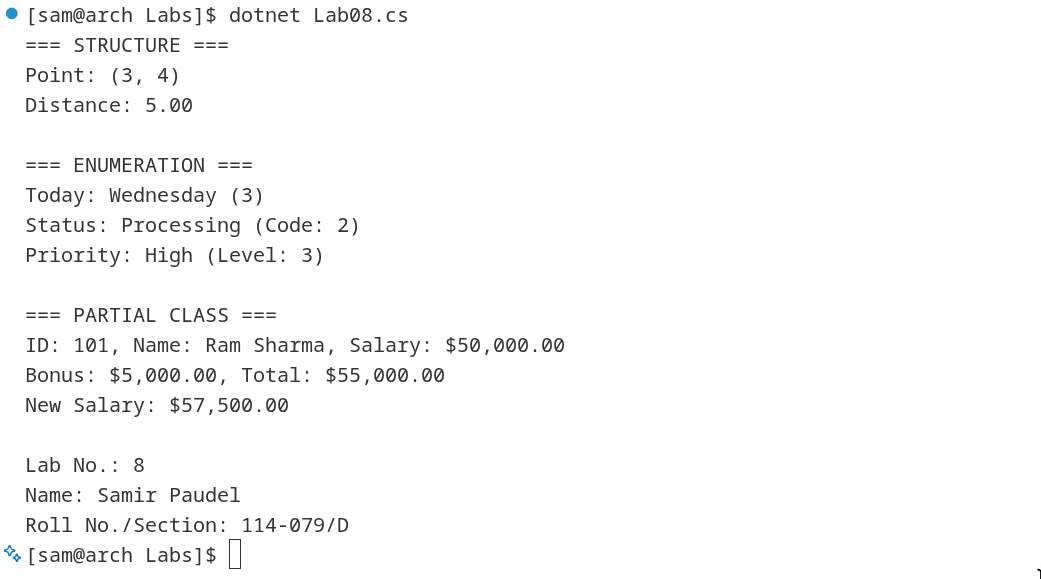
\includegraphics[width=0.6\linewidth]{lab08.png}
\end{figure}

\newpage

% ======================== LAB 9 ========================
\section*{Lab 9: Delegates, Multicast Delegates, and Events}

\subsection*{Title}
WAP to illustrate the concept of:\\
a) Delegate\\
b) Multicast delegate\\
c) Func Delegate\\
d) Action Delegate\\
e) Anonymous Method\\
f) Event in C\#

\subsection*{Theory}
\textbf{Delegate:} A type-safe function pointer that can reference methods with a specific signature.

\textbf{Multicast Delegate:} A delegate that can reference multiple methods. All referenced methods are called when the delegate is invoked.

\textbf{Func Delegate:} A built-in generic delegate that returns a value. Last type parameter is the return type.

\textbf{Action Delegate:} A built-in generic delegate that doesn't return a value (void).

\textbf{Anonymous Method:} A method without a name, defined using the \texttt{delegate} keyword.

\textbf{Event:} A mechanism for communication between objects based on the publisher-subscriber model. Events use delegates.

\subsection*{Code}
\begin{multicols}{2}
\begin{lstlisting}
using System;

// a) Delegate declaration
delegate int MathOperation(int a, int b);
delegate void DisplayMessage(string message);

// Event publisher class
class Button
{
    // f) Event declaration
    public event EventHandler Click;
    
    public void OnClick()
    {
        Console.WriteLine("Button clicked!");
        // Raise the event
        if (Click != null)
        {
            Click(this, EventArgs.Empty);
        }
    }
}

class Calculator
{
    // Methods for delegates
    public int Add(int a, int b)
    {
        return a + b;
    }
    
    public int Subtract(int a, int b)
    {
        return a - b;
    }
    
    public int Multiply(int a, int b)
    {
        return a * b;
    }
    
    public static void ShowResult(string message)
    {
        Console.WriteLine($"Result: {message}");
    }
}

class Program
{
    static void Main()
    {
        Calculator calc = new Calculator();
        
        // a) Delegate Demo
        Console.WriteLine("=== DELEGATE Demo ===\n");
        
        MathOperation operation = calc.Add;
        int result = operation(10, 5);
        Console.WriteLine($"10 + 5 = {result}");
        
        operation = calc.Subtract;
        result = operation(10, 5);
        Console.WriteLine($"10 - 5 = {result}");
        
        operation = calc.Multiply;
        result = operation(10, 5);
        Console.WriteLine($"10 * 5 = {result}");
        
        // b) Multicast Delegate Demo
        Console.WriteLine("\n=== MULTICAST DELEGATE Demo ===\n");
        
        DisplayMessage display = Calculator.ShowResult;
        display += msg => Console.WriteLine($"Display: {msg}");
        display += msg => Console.WriteLine($"Log: {msg}");
        
        Console.WriteLine("Calling multicast delegate:");
        display("Hello from multicast delegate");
        
        // c) Func Delegate Demo
        Console.WriteLine("\n=== FUNC DELEGATE Demo ===\n");
        
        // Func with two int parameters and int return
        Func<int, int, int> add = (x, y) => x + y;
        Func<int, int, int> multiply = (x, y) => x * y;
        
        Console.WriteLine($"Func Add: 15 + 10 = {add(15, 10)}");
        Console.WriteLine($"Func Multiply: 15 * 10 = {multiply(15, 10)}");
        
        // Func with string return
        Func<string, string> greet = name => $"Hello, {name}!";
        Console.WriteLine(greet("Ram"));
        
        // d) Action Delegate Demo
        Console.WriteLine("\n=== ACTION DELEGATE Demo ===\n");
        
        // Action with no return value
        Action<string> printMessage = message => 
            Console.WriteLine($"Action: {message}");
        printMessage("This is an Action delegate");
        
        Action<int, int> printSum = (a, b) => 
            Console.WriteLine($"Sum of {a} and {b} is {a + b}");
        printSum(20, 30);
        
        Action sayHello = () => Console.WriteLine("Hello from Action!");
        sayHello();
        
        // e) Anonymous Method Demo
        Console.WriteLine("\n=== ANONYMOUS METHOD Demo ===\n");
        
        MathOperation subtract = delegate(int x, int y)
        {
            Console.WriteLine($"Anonymous method: {x} - {y}");
            return x - y;
        };
        
        result = subtract(50, 20);
        Console.WriteLine($"Result: {result}");
        
        DisplayMessage anonymousDisplay = delegate(string msg)
        {
            Console.WriteLine($"Anonymous: {msg}");
            Console.WriteLine("This is an anonymous method!");
        };
        anonymousDisplay("Testing anonymous method");
        
        // f) Event Demo
        Console.WriteLine("\n=== EVENT Demo ===\n");
        
        Button button = new Button();
        
        // Subscribe to event
        button.Click += Button_Click;
        button.Click += (sender, e) => 
            Console.WriteLine("Event: Lambda handler executed");
        button.Click += delegate(object sender, EventArgs e)
        {
            Console.WriteLine("Event: Anonymous method handler executed");
        };
        
        // Trigger event
        button.OnClick();
        
        Console.WriteLine("\n=== Practical Example: Calculator with Delegates ===\n");
        
        Func<int, int, int> calculate;
        string operation_choice = "add";
        
        switch (operation_choice)
        {
            case "add":
                calculate = (a, b) => a + b;
                break;
            case "subtract":
                calculate = (a, b) => a - b;
                break;
            case "multiply":
                calculate = (a, b) => a * b;
                break;
            default:
                calculate = (a, b) => 0;
                break;
        }
        
        Console.WriteLine($"Result: {calculate(100, 50)}");
        
        Console.WriteLine("\nLab No.: 9");
        Console.WriteLine("Name: Samir Paudel");
        Console.WriteLine("Roll No./Section: 114-079/D");
    }
    
    // Event handler method
    static void Button_Click(object sender, EventArgs e)
    {
        Console.WriteLine("Event: Button_Click handler executed");
    }
}
\end{lstlisting}
\end{multicols}

\subsection*{Output}
\begin{figure}[h!]
    \raggedright
    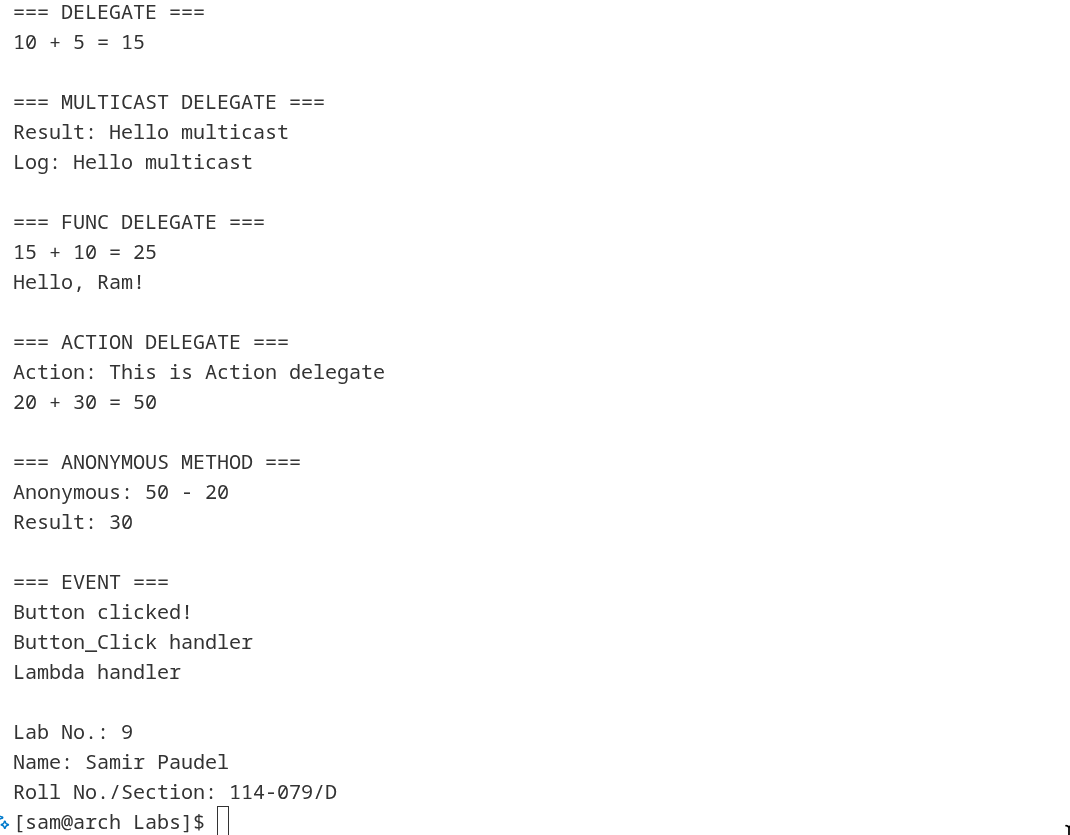
\includegraphics[width=0.6\linewidth]{lab09.png}
\end{figure}

\newpage

% ======================== LAB 10 ========================
\section*{Lab 10: Generic and Non-Generic Collections}

\subsection*{Title}
WAP which use any:\\
a) Non generic collection\\
b) Generic Collection

\subsection*{Theory}
\textbf{Non-Generic Collections:} Collections that store elements as \texttt{object} type. Found in \texttt{System.Collections} namespace. Examples: ArrayList, Hashtable, Stack, Queue.

\textbf{Generic Collections:} Type-safe collections that use generic type parameters. Found in \texttt{System.Collections.Generic} namespace. Examples: List<T>, Dictionary<TKey, TValue>, Stack<T>, Queue<T>.

Advantages of Generic Collections:
\begin{itemize}
    \item Type safety - No need for casting
    \item Better performance - No boxing/unboxing for value types
    \item Code reusability
    \item Compile-time type checking
\end{itemize}

\subsection*{Code}
\begin{multicols}{2}
\begin{lstlisting}
using System;
using System.Collections;           // Non-generic collections
using System.Collections.Generic;   // Generic collections

class Program
{
    static void Main()
    {
        // a) NON-GENERIC COLLECTIONS
        Console.WriteLine("=== NON-GENERIC COLLECTIONS ===\n");
        
        // ArrayList Demo
        Console.WriteLine("--- ArrayList Demo ---");
        ArrayList arrayList = new ArrayList();
        
        arrayList.Add(10);
        arrayList.Add("Hello");
        arrayList.Add(3.14);
        arrayList.Add(true);
        arrayList.Add("World");
        
        Console.WriteLine("ArrayList elements:");
        foreach (object item in arrayList)
        {
            Console.WriteLine($"{item} (Type: {item.GetType().Name})");
        }
        
        Console.WriteLine($"Count: {arrayList.Count}");
        Console.WriteLine($"Contains 'Hello': {arrayList.Contains("Hello")}");
        
        // Hashtable Demo
        Console.WriteLine("\n--- Hashtable Demo ---");
        Hashtable hashtable = new Hashtable();
        
        hashtable.Add("name", "Ram Sharma");
        hashtable.Add("age", 25);
        hashtable.Add("city", "Kathmandu");
        hashtable.Add("phone", "9841234567");
        
        Console.WriteLine("Hashtable elements:");
        foreach (DictionaryEntry entry in hashtable)
        {
            Console.WriteLine($"{entry.Key}: {entry.Value}");
        }
        
        Console.WriteLine($"Name: {hashtable["name"]}");
        
        // Stack (Non-Generic) Demo
        Console.WriteLine("\n--- Stack (Non-Generic) Demo ---");
        Stack stack = new Stack();
        
        stack.Push("First");
        stack.Push("Second");
        stack.Push("Third");
        stack.Push(100);
        
        Console.WriteLine("Stack elements (LIFO):");
        while (stack.Count > 0)
        {
            Console.WriteLine(stack.Pop());
        }
        
        // Queue (Non-Generic) Demo
        Console.WriteLine("\n--- Queue (Non-Generic) Demo ---");
        Queue queue = new Queue();
        
        queue.Enqueue("First");
        queue.Enqueue("Second");
        queue.Enqueue("Third");
        queue.Enqueue(200);
        
        Console.WriteLine("Queue elements (FIFO):");
        while (queue.Count > 0)
        {
            Console.WriteLine(queue.Dequeue());
        }
        
        // b) GENERIC COLLECTIONS
        Console.WriteLine("\n\n=== GENERIC COLLECTIONS ===\n");
        
        // List<T> Demo
        Console.WriteLine("--- List<T> Demo ---");
        List<int> numbers = new List<int>();
        
        numbers.Add(10);
        numbers.Add(20);
        numbers.Add(30);
        numbers.Add(40);
        numbers.Add(50);
        
        Console.WriteLine("List<int> elements:");
        foreach (int num in numbers)
        {
            Console.WriteLine(num);
        }
        
        numbers.Remove(30);
        Console.WriteLine($"After removing 30, Count: {numbers.Count}");
        
        List<string> names = new List<string> 
            { "Ram", "Sita", "Hari", "Gita" };
        Console.WriteLine("\nList<string> elements:");
        names.ForEach(name => Console.WriteLine(name));
        
        // Dictionary<TKey, TValue> Demo
        Console.WriteLine("\n--- Dictionary<TKey, TValue> Demo ---");
        Dictionary<string, string> dictionary = new Dictionary<string, string>();
        
        dictionary.Add("NPL", "Nepal");
        dictionary.Add("IND", "India");
        dictionary.Add("USA", "United States");
        dictionary.Add("UK", "United Kingdom");
        
        Console.WriteLine("Dictionary elements:");
        foreach (KeyValuePair<string, string> kvp in dictionary)
        {
            Console.WriteLine($"{kvp.Key}: {kvp.Value}");
        }
        
        Console.WriteLine($"\nNPL stands for: {dictionary["NPL"]}");
        
        // Dictionary with int key
        Dictionary<int, string> studentDict = new Dictionary<int, string>();
        studentDict.Add(101, "Ram Kumar");
        studentDict.Add(102, "Sita Devi");
        studentDict.Add(103, "Hari Prasad");
        
        Console.WriteLine("\nStudent Dictionary:");
        foreach (var student in studentDict)
        {
            Console.WriteLine($"Roll {student.Key}: {student.Value}");
        }
        
        // Stack<T> Demo
        Console.WriteLine("\n--- Stack<T> (Generic) Demo ---");
        Stack<string> genericStack = new Stack<string>();
        
        genericStack.Push("Page 1");
        genericStack.Push("Page 2");
        genericStack.Push("Page 3");
        genericStack.Push("Page 4");
        
        Console.WriteLine("Stack<string> elements (LIFO):");
        Console.WriteLine($"Peek: {genericStack.Peek()}");
        while (genericStack.Count > 0)
        {
            Console.WriteLine(genericStack.Pop());
        }
        
        // Queue<T> Demo
        Console.WriteLine("\n--- Queue<T> (Generic) Demo ---");
        Queue<int> genericQueue = new Queue<int>();
        
        genericQueue.Enqueue(100);
        genericQueue.Enqueue(200);
        genericQueue.Enqueue(300);
        genericQueue.Enqueue(400);
        
        Console.WriteLine("Queue<int> elements (FIFO):");
        Console.WriteLine($"Peek: {genericQueue.Peek()}");
        while (genericQueue.Count > 0)
        {
            Console.WriteLine(genericQueue.Dequeue());
        }
        
        // HashSet<T> Demo
        Console.WriteLine("\n--- HashSet<T> Demo ---");
        HashSet<int> hashSet = new HashSet<int>();
        
        hashSet.Add(10);
        hashSet.Add(20);
        hashSet.Add(30);
        hashSet.Add(20);  // Duplicate, won't be added
        hashSet.Add(40);
        
        Console.WriteLine("HashSet<int> elements (no duplicates):");
        foreach (int item in hashSet)
        {
            Console.WriteLine(item);
        }
        Console.WriteLine($"Count: {hashSet.Count}");
        
        Console.WriteLine("\nLab No.: 10");
        Console.WriteLine("Name: Samir Paudel");
        Console.WriteLine("Roll No./Section: 114-079/D");
    }
}
\end{lstlisting}
\end{multicols}

\subsection*{Output}
\begin{figure}[h!]
    \raggedright
    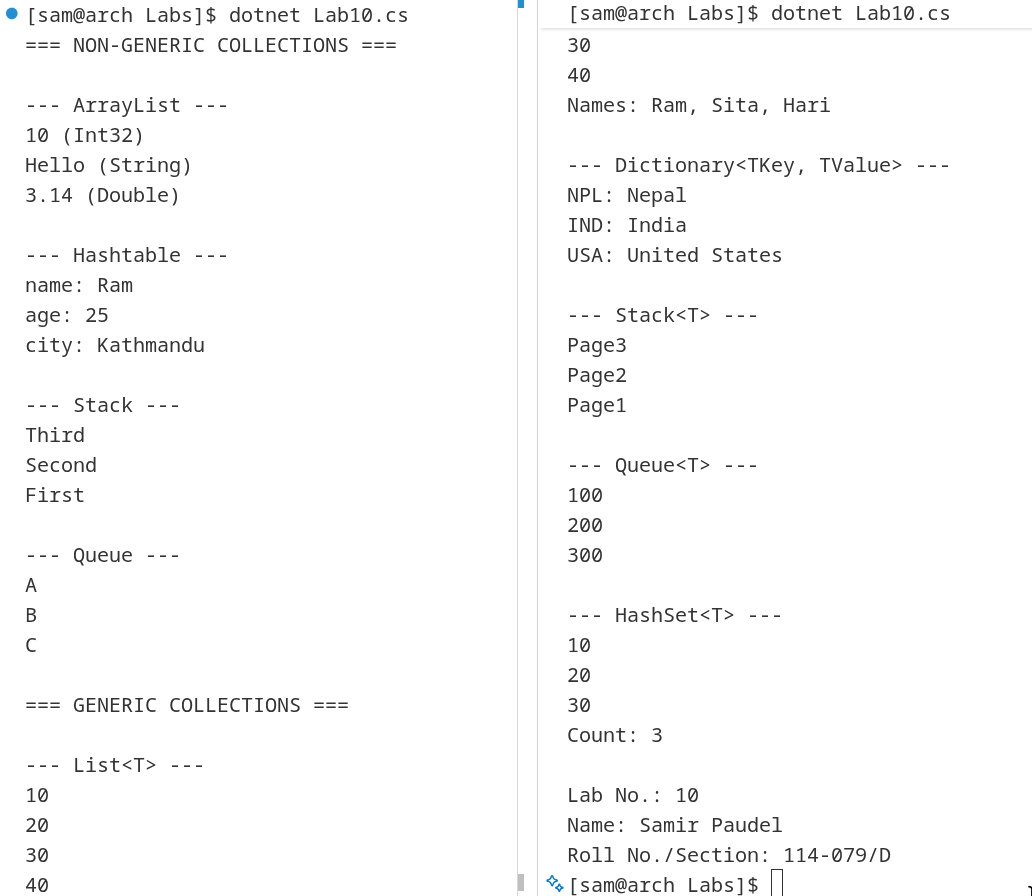
\includegraphics[width=0.45\linewidth]{lab10.png}
\end{figure}

\newpage

% ======================== LAB 11 ========================
\section*{Lab 11: Generic Class with Generic Field and Method}

\subsection*{Title}
Program to demonstrate the use of Generic Class with Generic field and method.

\subsection*{Theory}
\textbf{Generic Classes} use type parameters (T) to create type-safe, reusable code without boxing/unboxing overhead. They can have generic fields, properties, and methods.

\textbf{Type Constraints} restrict generic type parameters using the \texttt{where} keyword. Common constraints: \texttt{struct} (value types), \texttt{class} (reference types), \texttt{new()} (parameterless constructor).

Benefits: Type safety at compile time, code reusability, better performance, and support for multiple type parameters.

\subsection*{Code}
\begin{multicols}{2}
\begin{lstlisting}
using System;

// Generic Class with Generic Field and Method
class Box<T>
{
  // Generic field
  private T item;
  
  public void SetItem(T value)
  {
    item = value;
    Console.WriteLine($"Item set: {item}");
  }
  
  public T GetItem()
  {
    return item;
  }
  
  // Generic method
  public void Display<U>(U data)
  {
    Console.WriteLine($"Generic Method - Type: {typeof(U).Name}, Value: {data}");
  }
}

// Generic class with multiple type parameters
class Pair<T1, T2>
{
  public T1 First { get; set; }
  public T2 Second { get; set; }
  
  public Pair(T1 first, T2 second)
  {
    First = first;
    Second = second;
  }
  
  public void DisplayPair()
  {
    Console.WriteLine($"Pair: ({First}, {Second})");
  }
  
  // Generic method with constraint
  public void Swap<T>(ref T a, ref T b)
  {
    T temp = a;
    a = b;
    b = temp;
  }
}

// Generic class with constraints
class Calculator<T> where T : struct
{
  public void Add(T a, T b)
  {
    dynamic x = a;
    dynamic y = b;
    Console.WriteLine($"{a} + {b} = {x + y}");
  }
}

class Program
{
  static void Main()
  {
    Console.WriteLine("=== Generic Class with Generic Field ===");
    Box<int> intBox = new Box<int>();
    intBox.SetItem(100);
    Console.WriteLine($"Retrieved: {intBox.GetItem()}");
    
    Console.WriteLine();
    Box<string> strBox = new Box<string>();
    strBox.SetItem("Hello Generic");
    Console.WriteLine($"Retrieved: {strBox.GetItem()}");
    
    Console.WriteLine("\n=== Generic Method ===");
    intBox.Display(42);
    intBox.Display("String value");
    intBox.Display(3.14);
    
    Console.WriteLine("\n=== Generic Class with Multiple Parameters ===");
    Pair<int, string> pair1 = new Pair<int, string>(1, "One");
    pair1.DisplayPair();
    
    Pair<string, double> pair2 = new Pair<string, double>("PI", 3.14159);
    pair2.DisplayPair();
    
    Console.WriteLine("\n=== Generic Method with Swap ===");
    int a = 10, b = 20;
    Console.WriteLine($"Before: a={a}, b={b}");
    pair1.Swap(ref a, ref b);
    Console.WriteLine($"After: a={a}, b={b}");
    
    Console.WriteLine("\n=== Generic Class with Constraints ===");
    Calculator<int> calc = new Calculator<int>();
    calc.Add(15, 25);
    
    Calculator<double> calcDouble = new Calculator<double>();
    calcDouble.Add(5.5, 4.5);
    
    Console.WriteLine("\nLab No.: 11");
    Console.WriteLine("Name: Samir Paudel");
    Console.WriteLine("Roll No./Section: 114-079/D");
  }
}
\end{lstlisting}
\end{multicols}

\subsection*{Output}
\begin{figure}[h!]
    \raggedright
    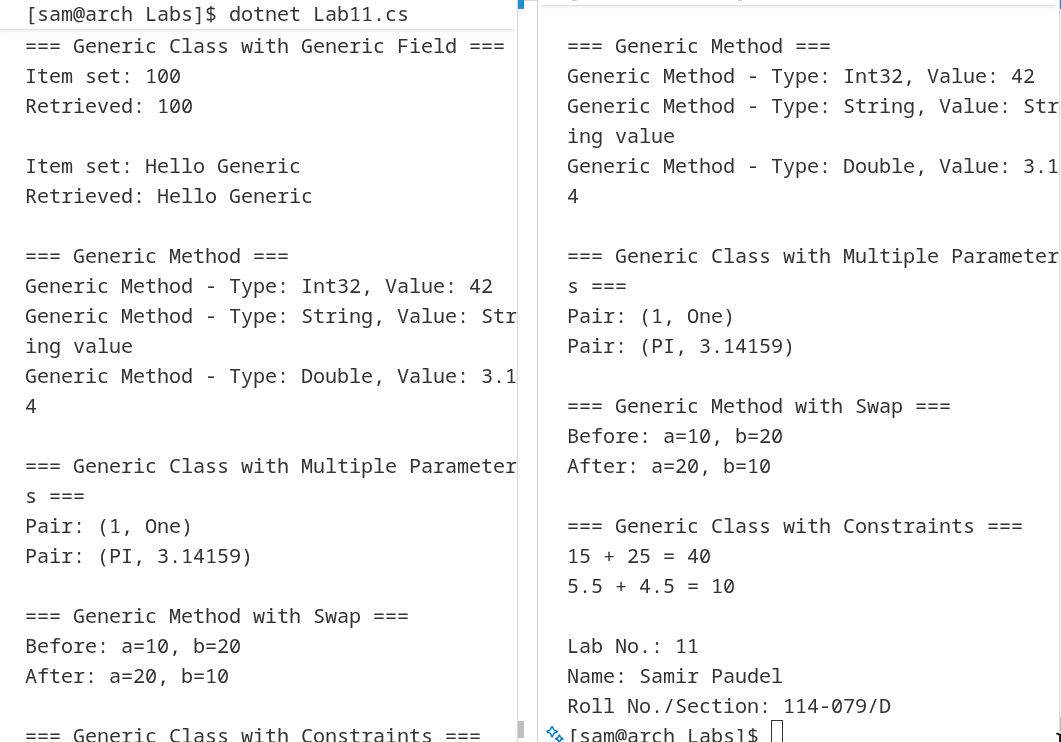
\includegraphics[width=0.7\linewidth]{lab11.png}
\end{figure}

\newpage

% ======================== LAB 12 ========================
\section*{Lab 12: File Input/Output}

\subsection*{Title}
WAP to take input from keyboard and write them to a file

\subsection*{Theory}
\textbf{File I/O} in C\# uses the \texttt{System.IO} namespace. \texttt{StreamWriter} writes text to files, \texttt{StreamReader} reads from files. The \texttt{using} statement ensures proper resource disposal.

\texttt{File} class provides static methods like \texttt{ReadAllText()}, \texttt{WriteAllText()}. StreamWriter constructor with second parameter \texttt{true} enables append mode.

Best practice: Use \texttt{using} blocks for automatic file closure and resource cleanup.

\subsection*{Code}
\begin{multicols}{2}
\begin{lstlisting}
using System;
using System.IO;

class Program
{
  static void Main()
  {
    Console.WriteLine("=== Write Input to File ===\n");
    
    string fileName = "student_data.txt";
    
    try
    {
      // Take input from keyboard
      Console.Write("Enter your name: ");
      string name = Console.ReadLine();
      
      Console.Write("Enter your roll number: ");
      string rollNo = Console.ReadLine();
      
      Console.Write("Enter your age: ");
      string age = Console.ReadLine();
      
      Console.Write("Enter your address: ");
      string address = Console.ReadLine();
      
      // Write to file
      using (StreamWriter writer = new StreamWriter(fileName))
      {
        writer.WriteLine("Student Information");
        writer.WriteLine("===================");
        writer.WriteLine($"Name: {name}");
        writer.WriteLine($"Roll No: {rollNo}");
        writer.WriteLine($"Age: {age}");
        writer.WriteLine($"Address: {address}");
        writer.WriteLine();
        writer.WriteLine("Lab No.: 12");
        writer.WriteLine("Name: Samir Paudel");
        writer.WriteLine("Roll No./Section: 114-079/D");
      }
      
      Console.WriteLine($"\nData written to {fileName} successfully!");
      
      // Read and display file contents
      Console.WriteLine("\n=== File Contents ===\n");
      using (StreamReader reader = new StreamReader(fileName))
      {
        string content = reader.ReadToEnd();
        Console.WriteLine(content);
      }
      
      // Append more data
      Console.WriteLine("\n=== Append Mode ===");
      Console.Write("\nEnter additional comment: ");
      string comment = Console.ReadLine();
      
      using (StreamWriter writer = new StreamWriter(fileName, true))
      {
        writer.WriteLine($"\nComment: {comment}");
        writer.WriteLine($"Date: {DateTime.Now}");
      }
      
      Console.WriteLine("Comment appended successfully!");
      
      // Display final contents
      Console.WriteLine("\n=== Final File Contents ===\n");
      string finalContent = File.ReadAllText(fileName);
      Console.WriteLine(finalContent);
    }
    catch (Exception ex)
    {
      Console.WriteLine($"Error: {ex.Message}");
    }
    
    Console.WriteLine("\nLab No.: 12");
    Console.WriteLine("Name: Samir Paudel");
    Console.WriteLine("Roll No./Section: 114-079/D");
  }
}
\end{lstlisting}
\end{multicols}

\subsection*{Output}
\begin{figure}[h!]
    \raggedright
    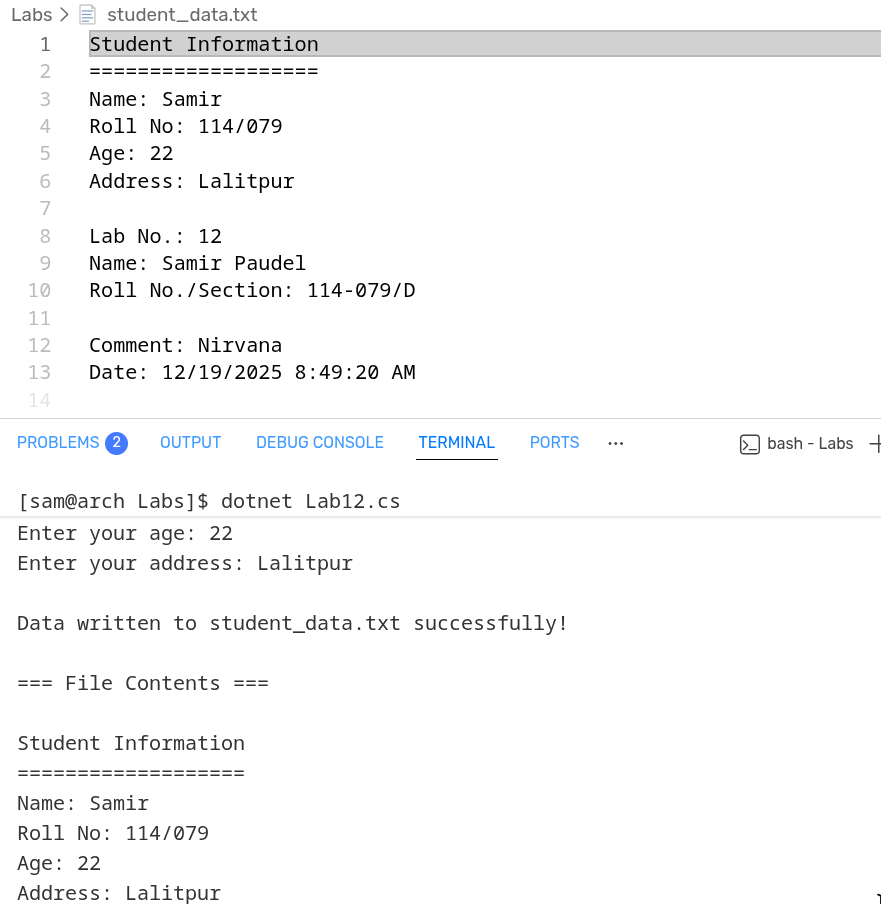
\includegraphics[width=0.7\linewidth]{lab12.png}
\end{figure}

\newpage

% ======================== LAB 13 ========================
\section*{Lab 13: LINQ (Language Integrated Query)}

\subsection*{Title}
WAP to demonstrate the concept of LINQ

\subsection*{Theory}
\textbf{LINQ (Language Integrated Query)} provides query capabilities directly in C\#. It works with collections, databases, XML, and more.

Key operations: \texttt{Where} (filter), \texttt{Select} (project), \texttt{OrderBy} (sort), \texttt{GroupBy} (group), aggregates (\texttt{Sum}, \texttt{Average}, \texttt{Count}, \texttt{Max}, \texttt{Min}).

Two syntaxes: Query syntax (SQL-like) and Method syntax (using lambda expressions). Both produce same results.

\subsection*{Code}
\begin{multicols}{2}
\begin{lstlisting}
using System;
using System.Linq;
using System.Collections.Generic;

class Student
{
  public int RollNo { get; set; }
  public string Name { get; set; }
  public int Age { get; set; }
  public double Marks { get; set; }
  public string City { get; set; }
}

class Program
{
  static void Main()
  {
    // Sample data
    List<Student> students = new List<Student>
    {
      new Student { RollNo = 1, Name = "Ram", Age = 20, Marks = 85, City = "Kathmandu" },
      new Student { RollNo = 2, Name = "Sita", Age = 19, Marks = 92, City = "Pokhara" },
      new Student { RollNo = 3, Name = "Hari", Age = 21, Marks = 78, City = "Kathmandu" },
      new Student { RollNo = 4, Name = "Gita", Age = 20, Marks = 88, City = "Lalitpur" },
      new Student { RollNo = 5, Name = "Shyam", Age = 22, Marks = 95, City = "Pokhara" }
    };
    
    int[] numbers = { 5, 2, 8, 1, 9, 3, 7, 4, 6 };
    
    Console.WriteLine("=== LINQ - Where (Filtering) ===");
    var passedStudents = students.Where(s => s.Marks >= 80);
    foreach (var s in passedStudents)
      Console.WriteLine($"{s.Name}: {s.Marks}");
    
    Console.WriteLine("\n=== LINQ - Select (Projection) ===");
    var studentNames = students.Select(s => s.Name);
    Console.WriteLine("Names: " + string.Join(", ", studentNames));
    
    Console.WriteLine("\n=== LINQ - OrderBy ===");
    var sortedByMarks = students.OrderByDescending(s => s.Marks);
    foreach (var s in sortedByMarks)
      Console.WriteLine($"{s.Name}: {s.Marks}");
    
    Console.WriteLine("\n=== LINQ - GroupBy ===");
    var studentsByCity = students.GroupBy(s => s.City);
    foreach (var group in studentsByCity)
    {
      Console.WriteLine($"\n{group.Key}:");
      foreach (var s in group)
        Console.WriteLine($"  {s.Name}");
    }
    
    Console.WriteLine("\n=== LINQ - Aggregate Functions ===");
    Console.WriteLine($"Total Students: {students.Count()}");
    Console.WriteLine($"Average Marks: {students.Average(s => s.Marks):F2}");
    Console.WriteLine($"Highest Marks: {students.Max(s => s.Marks)}");
    Console.WriteLine($"Lowest Marks: {students.Min(s => s.Marks)}");
    Console.WriteLine($"Sum of Marks: {students.Sum(s => s.Marks)}");
    
    Console.WriteLine("\n=== LINQ - First, Last, Single ===");
    var firstStudent = students.First();
    Console.WriteLine($"First: {firstStudent.Name}");
    
    var topStudent = students.First(s => s.Marks > 90);
    Console.WriteLine($"First with >90: {topStudent.Name}");
    
    Console.WriteLine("\n=== LINQ - Query Syntax ===");
    var query = from s in students
                where s.Age >= 20 && s.Marks >= 85
                orderby s.Marks descending
                select new { s.Name, s.Marks, s.City };
    
    foreach (var item in query)
      Console.WriteLine($"{item.Name} ({item.City}): {item.Marks}");
    
    Console.WriteLine("\n=== LINQ on Arrays ===");
    var evenNumbers = numbers.Where(n => n % 2 == 0);
    Console.WriteLine("Even: " + string.Join(", ", evenNumbers));
    
    var sortedNumbers = numbers.OrderBy(n => n);
    Console.WriteLine("Sorted: " + string.Join(", ", sortedNumbers));
    
    Console.WriteLine("\n=== LINQ - Any, All ===");
    Console.WriteLine($"Any student with 100? {students.Any(s => s.Marks == 100)}");
    Console.WriteLine($"All students passed (>50)? {students.All(s => s.Marks > 50)}");
    
    Console.WriteLine("\nLab No.: 13");
    Console.WriteLine("Name: Samir Paudel");
    Console.WriteLine("Roll No./Section: 114-079/D");
  }
}
\end{lstlisting}
\end{multicols}

\subsection*{Output}
\begin{figure}[h!]
    \raggedright
    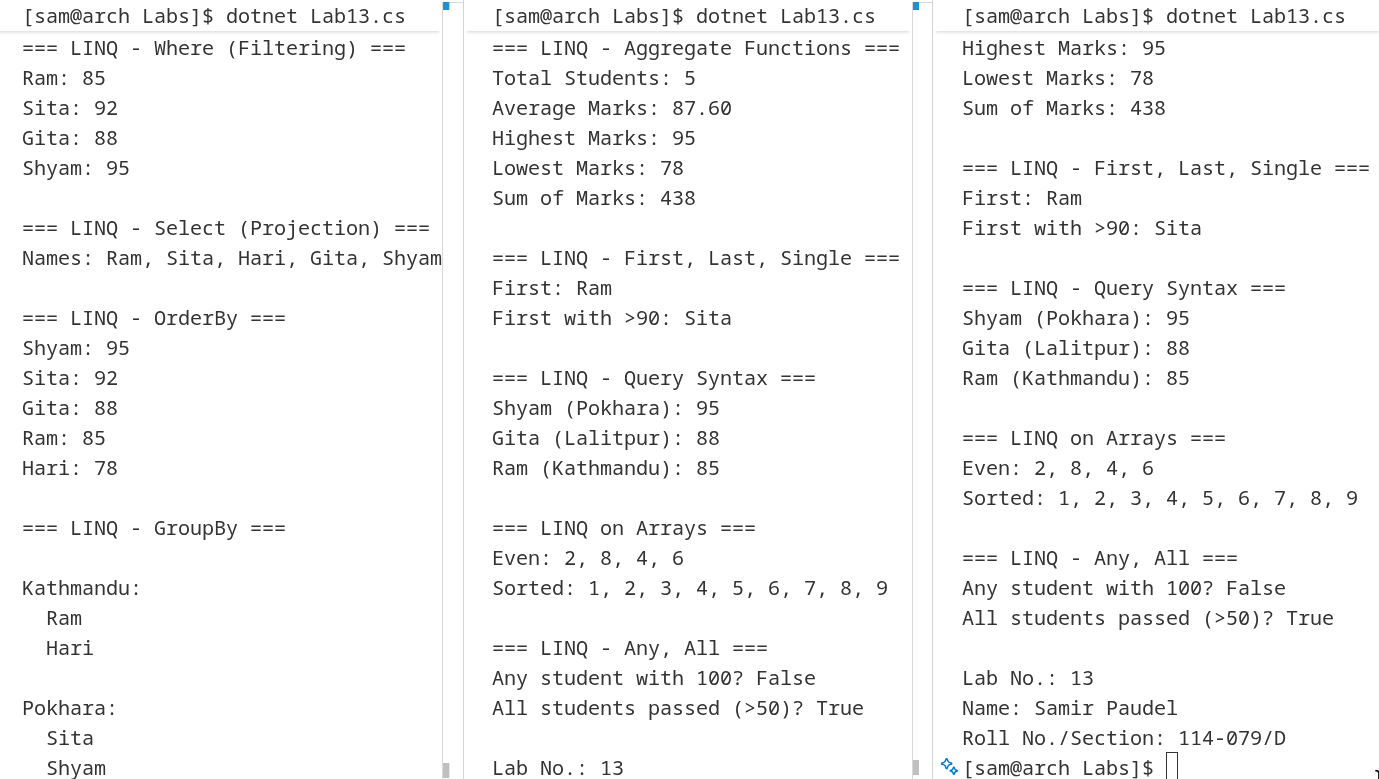
\includegraphics[width=0.7\linewidth]{lab13.png}
\end{figure}

\newpage

% ======================== LAB 14 ========================
\section*{Lab 14: Lambda Expressions}

\subsection*{Title}
WAP to demonstrate Lambda Expressions in C\#.

\subsection*{Theory}
\textbf{Lambda Expressions} are anonymous functions using the \texttt{=>} operator (read as ``goes to''). Syntax: \texttt{(parameters) => expression} or \texttt{(parameters) => \{ statements \}}.

Commonly used with LINQ, delegates (\texttt{Func}, \texttt{Action}), and event handlers. Provide concise way to write inline functions.

Types: Expression lambdas (single expression) and Statement lambdas (code block with braces).

\subsection*{Code}
\begin{multicols}{2}
\begin{lstlisting}
using System;
using System.Collections.Generic;
using System.Linq;

class Program
{
  static void Main()
  {
    Console.WriteLine("=== Lambda Expression - Basic ===");
    
    // Lambda with no parameters
    Action greet = () => Console.WriteLine("Hello from Lambda!");
    greet();
    
    // Lambda with one parameter
    Action<string> sayHello = name => Console.WriteLine($"Hello, {name}!");
    sayHello("Ram");
    
    // Lambda with multiple parameters
    Func<int, int, int> add = (a, b) => a + b;
    Console.WriteLine($"10 + 5 = {add(10, 5)}");
    
    Func<int, int, int> multiply = (x, y) => x * y;
    Console.WriteLine($"10 * 5 = {multiply(10, 5)}");
    
    Console.WriteLine("\n=== Lambda with Collections ===");
    List<int> numbers = new List<int> { 1, 2, 3, 4, 5, 6, 7, 8, 9, 10 };
    
    // Filter using lambda
    var evenNumbers = numbers.Where(n => n % 2 == 0).ToList();
    Console.WriteLine("Even: " + string.Join(", ", evenNumbers));
    
    // Transform using lambda
    var squares = numbers.Select(n => n * n).ToList();
    Console.WriteLine("Squares: " + string.Join(", ", squares));
    
    // Sort using lambda
    List<string> names = new List<string> { "Ram", "Hari", "Sita", "Gita" };
    var sortedNames = names.OrderBy(n => n.Length).ToList();
    Console.WriteLine("Sorted by length: " + string.Join(", ", sortedNames));
    
    Console.WriteLine("\n=== Lambda for Filtering ===");
    var greaterThan5 = numbers.Where(n => n > 5).ToList();
    Console.WriteLine("Greater than 5: " + string.Join(", ", greaterThan5));
    
    Console.WriteLine("\n=== Lambda with Objects ===");
    List<Person> people = new List<Person>
    {
      new Person { Name = "Ram", Age = 25, Salary = 50000 },
      new Person { Name = "Sita", Age = 30, Salary = 60000 },
      new Person { Name = "Hari", Age = 22, Salary = 45000 },
      new Person { Name = "Gita", Age = 28, Salary = 55000 }
    };
    
    // Filter
    var youngPeople = people.Where(p => p.Age < 28).ToList();
    Console.WriteLine("\nAge < 28:");
    youngPeople.ForEach(p => Console.WriteLine($"{p.Name}: {p.Age}"));
    
    // Select specific properties
    var salaries = people.Select(p => p.Salary).ToList();
    Console.WriteLine("\nSalaries: " + string.Join(", ", salaries));
    
    // Order by
    var orderedBySalary = people.OrderByDescending(p => p.Salary).ToList();
    Console.WriteLine("\nOrdered by Salary:");
    orderedBySalary.ForEach(p => Console.WriteLine($"{p.Name}: {p.Salary}"));
    
    Console.WriteLine("\n=== Lambda - Multiple Statements ===");
    Func<int, int, string> compare = (a, b) =>
    {
      if (a > b) return $"{a} is greater";
      else if (a < b) return $"{b} is greater";
      else return "Both are equal";
    };
    Console.WriteLine(compare(10, 5));
    Console.WriteLine(compare(3, 8));
    
    Console.WriteLine("\n=== Lambda - Aggregate Operations ===");
    int sum = numbers.Sum();
    double average = numbers.Average();
    int max = numbers.Max();
    int min = numbers.Min();
    
    Console.WriteLine($"Sum: {sum}");
    Console.WriteLine($"Average: {average}");
    Console.WriteLine($"Max: {max}");
    Console.WriteLine($"Min: {min}");
    
    // Custom aggregate
    var totalSalary = people.Sum(p => p.Salary);
    Console.WriteLine($"\nTotal Salary: {totalSalary}");
    
    Console.WriteLine("\n=== Lambda - Find ===");
    var firstHighEarner = people.FirstOrDefault(p => p.Salary > 55000);
    if (firstHighEarner != null)
      Console.WriteLine($"First high earner: {firstHighEarner.Name}");
    
    Console.WriteLine("\nLab No.: 14");
    Console.WriteLine("Name: Samir Paudel");
    Console.WriteLine("Roll No./Section: 114-079/D");
  }
}

class Person
{
  public string Name { get; set; }
  public int Age { get; set; }
  public double Salary { get; set; }
}
\end{lstlisting}
\end{multicols}

\subsection*{Output}
\begin{figure}[h!]
    \raggedright
    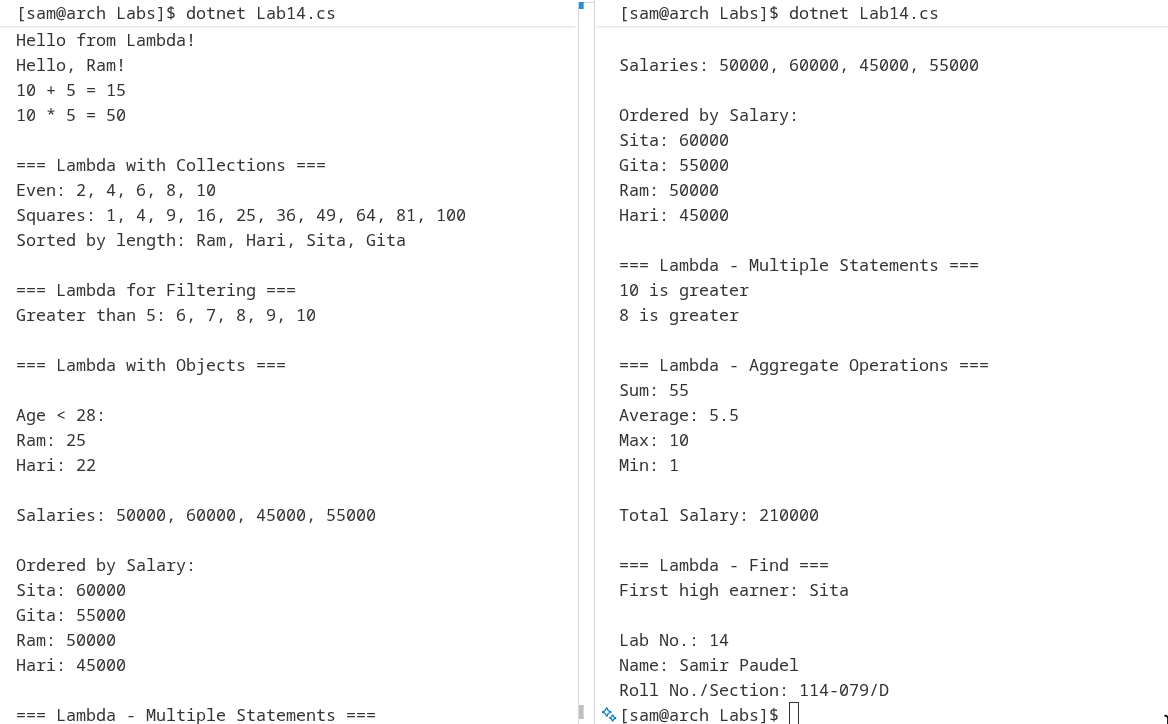
\includegraphics[width=0.7\linewidth]{lab14.png}
\end{figure}

\newpage

% ======================== LAB 15 ========================
\section*{Lab 15: Exception Handling}

\subsection*{Title}
WAP to:\\
a) demonstrate exception handling in C\# using try, catch and finally blocks\\
b) deal with throw keyword in exception handling\\
c) demonstrate custom exception handling

\subsection*{Theory}
\textbf{Exception Handling} uses try-catch-finally blocks. \texttt{try} contains code that may throw exceptions. \texttt{catch} handles specific exception types. \texttt{finally} executes regardless of exception occurrence.

\texttt{throw} keyword raises exceptions explicitly. Custom exceptions inherit from \texttt{Exception} class and can have custom properties for additional information.

Multiple catch blocks handle different exception types. Specific exceptions should be caught before general ones.

\subsection*{Code}
\begin{multicols}{2}
\begin{lstlisting}
using System;

// Custom Exception
class InvalidAgeException : Exception
{
  public InvalidAgeException(string message) : base(message) { }
}

class InsufficientBalanceException : Exception
{
  public double Balance { get; set; }
  public double RequestedAmount { get; set; }
  
  public InsufficientBalanceException(string message, double balance, double requested) 
    : base(message)
  {
    Balance = balance;
    RequestedAmount = requested;
  }
}

class BankAccount
{
  private double balance;
  
  public BankAccount(double initialBalance)
  {
    balance = initialBalance;
  }
  
  public void Withdraw(double amount)
  {
    if (amount > balance)
      throw new InsufficientBalanceException(
        "Insufficient balance!", balance, amount);
    
    balance -= amount;
    Console.WriteLine($"Withdrawn: {amount}, Balance: {balance}");
  }
}

class Program
{
  static void Main()
  {
    Console.WriteLine("=== Try-Catch-Finally ===\n");
    
    try
    {
      Console.Write("Enter first number: ");
      int num1 = int.Parse(Console.ReadLine());
      
      Console.Write("Enter second number: ");
      int num2 = int.Parse(Console.ReadLine());
      
      int result = num1 / num2;
      Console.WriteLine($"Result: {num1} / {num2} = {result}");
    }
    catch (DivideByZeroException ex)
    {
      Console.WriteLine($"Error: {ex.Message}");
    }
    catch (FormatException ex)
    {
      Console.WriteLine($"Invalid input: {ex.Message}");
    }
    catch (Exception ex)
    {
      Console.WriteLine($"General Error: {ex.Message}");
    }
    finally
    {
      Console.WriteLine("Finally block executed - Cleanup done");
    }
    
    Console.WriteLine("\n=== Throw Keyword ===\n");
    
    try
    {
      ValidateAge(15);
    }
    catch (InvalidAgeException ex)
    {
      Console.WriteLine($"Custom Exception: {ex.Message}");
    }
    
    Console.WriteLine("\n=== Multiple Catch Blocks ===\n");
    
    try
    {
      int[] numbers = { 1, 2, 3 };
      Console.WriteLine(numbers[5]); // Index out of range
    }
    catch (IndexOutOfRangeException ex)
    {
      Console.WriteLine($"Index Error: {ex.Message}");
    }
    catch (Exception ex)
    {
      Console.WriteLine($"Error: {ex.Message}");
    }
    
    Console.WriteLine("\n=== Custom Exception with Properties ===\n");
    
    BankAccount account = new BankAccount(5000);
    
    try
    {
      account.Withdraw(3000);
      account.Withdraw(3000); // This will throw exception
    }
    catch (InsufficientBalanceException ex)
    {
      Console.WriteLine($"Error: {ex.Message}");
      Console.WriteLine($"Balance: {ex.Balance}");
      Console.WriteLine($"Requested: {ex.RequestedAmount}");
      Console.WriteLine($"Shortage: {ex.RequestedAmount - ex.Balance}");
    }
    
    Console.WriteLine("\n=== Nested Try-Catch ===\n");
    
    try
    {
      try
      {
        int x = 10 / 0;
      }
      catch (DivideByZeroException)
      {
        Console.WriteLine("Inner catch: Division by zero");
        throw; // Re-throw the exception
      }
    }
    catch (Exception ex)
    {
      Console.WriteLine($"Outer catch: {ex.GetType().Name}");
    }
    
    Console.WriteLine("\n=== Exception with Stack Trace ===\n");
    
    try
    {
      Method1();
    }
    catch (Exception ex)
    {
      Console.WriteLine($"Exception: {ex.Message}");
      Console.WriteLine($"Source: {ex.Source}");
      Console.WriteLine("Stack Trace:");
      Console.WriteLine(ex.StackTrace);
    }
    
    Console.WriteLine("\nLab No.: 15");
    Console.WriteLine("Name: Samir Paudel");
    Console.WriteLine("Roll No./Section: 114-079/D");
  }
  
  static void ValidateAge(int age)
  {
    if (age < 18)
      throw new InvalidAgeException($"Age {age} is below 18!");
    
    Console.WriteLine($"Age {age} is valid");
  }
  
  static void Method1()
  {
    Method2();
  }
  
  static void Method2()
  {
    Method3();
  }
  
  static void Method3()
  {
    throw new Exception("Error in Method3");
  }
}
\end{lstlisting}
\end{multicols}

\subsection*{Output}
\begin{figure}[h!]
    \raggedright
    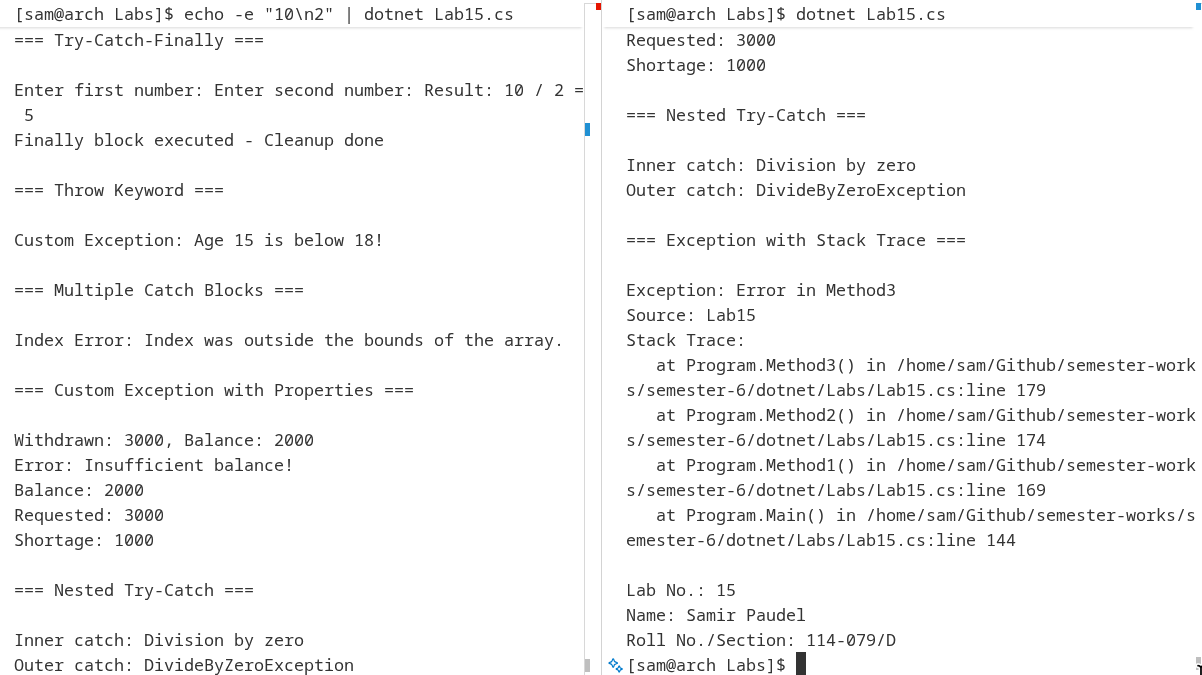
\includegraphics[width=0.7\linewidth]{lab15.png}
\end{figure}

\newpage

% ======================== LAB 16 ========================
\section*{Lab 16: Attributes in C\#}

\subsection*{Title}
WAP to:\\
a) use built-in attributes in C\#\\
b) create and use custom attribute in C\#

\subsection*{Theory}
\textbf{Attributes} add metadata to code elements (classes, methods, properties). They don't affect program logic but provide information for reflection, serialization, etc.

Built-in attributes: \texttt{[Obsolete]}, \texttt{[Serializable]}, \texttt{[Conditional]}. Custom attributes inherit from \texttt{Attribute} class.

\texttt{AttributeUsage} controls where attributes can be applied. Reflection (\texttt{GetCustomAttributes}) reads attribute data at runtime.

\subsection*{Code}
\begin{multicols}{2}
\begin{lstlisting}
using System;

// Custom Attribute
[AttributeUsage(AttributeTargets.Class | AttributeTargets.Method, AllowMultiple = true)]
class DeveloperInfoAttribute : Attribute
{
  public string Name { get; set; }
  public string Date { get; set; }
  public string Version { get; set; }
  
  public DeveloperInfoAttribute(string name)
  {
    Name = name;
    Date = DateTime.Now.ToShortDateString();
  }
  
  public void DisplayInfo()
  {
    Console.WriteLine($"Developer: {Name}");
    Console.WriteLine($"Date: {Date}");
    Console.WriteLine($"Version: {Version ?? "1.0"}");
  }
}

[AttributeUsage(AttributeTargets.Method)]
class TestMethodAttribute : Attribute
{
  public string Description { get; set; }
  
  public TestMethodAttribute(string description)
  {
    Description = description;
  }
}

// Using Built-in Attributes
[Serializable]
[DeveloperInfo("Samir Paudel", Version = "2.0")]
class Student
{
  public string Name { get; set; }
  public int Age { get; set; }
  
  [Obsolete("Use GetFullInfo() instead")]
  public void DisplayInfo()
  {
    Console.WriteLine($"{Name}, Age: {Age}");
  }
  
  [DeveloperInfo("Samir", Version = "1.5")]
  [TestMethod("Tests full information display")]
  public void GetFullInfo()
  {
    Console.WriteLine($"Student: {Name}, Age: {Age}");
  }
}

class Calculator
{
  [Obsolete("This method is deprecated. Use AddNumbers instead.", true)]
  public int Add(int a, int b)
  {
    return a + b;
  }
  
  public int AddNumbers(int a, int b)
  {
    return a + b;
  }
  
  [DeveloperInfo("Ram", Version = "2.1")]
  [TestMethod("Tests multiplication")]
  public int Multiply(int a, int b)
  {
    return a * b;
  }
}

class Program
{
  static void Main()
  {
    Console.WriteLine("=== Built-in Attributes ===\n");
    
    Student student = new Student { Name = "Ram", Age = 20 };
    
    // Using obsolete method (generates warning)
    student.DisplayInfo();
    
    // Using new method
    student.GetFullInfo();
    
    Console.WriteLine("\n=== Custom Attributes ===\n");
    
    // Reading custom attributes from class
    Type studentType = typeof(Student);
    var classAttributes = studentType.GetCustomAttributes(typeof(DeveloperInfoAttribute), false);
    
    Console.WriteLine($"Class: {studentType.Name}");
    foreach (DeveloperInfoAttribute attr in classAttributes)
    {
      attr.DisplayInfo();
      Console.WriteLine();
    }
    
    // Reading attributes from methods
    var methods = studentType.GetMethods();
    
    foreach (var method in methods)
    {
      var devAttrs = method.GetCustomAttributes(typeof(DeveloperInfoAttribute), false);
      var testAttrs = method.GetCustomAttributes(typeof(TestMethodAttribute), false);
      
      if (devAttrs.Length > 0 || testAttrs.Length > 0)
      {
        Console.WriteLine($"Method: {method.Name}");
        
        foreach (DeveloperInfoAttribute attr in devAttrs)
        {
          Console.Write("  ");
          attr.DisplayInfo();
        }
        
        foreach (TestMethodAttribute attr in testAttrs)
        {
          Console.WriteLine($"  Test: {attr.Description}");
        }
        
        Console.WriteLine();
      }
    }
    
    Console.WriteLine("=== Other Built-in Attributes ===\n");
    
    // Conditional attribute example
    TestConditionalMethod();
    
    Console.WriteLine("\n=== Reading All Attributes ===\n");
    
    Type calcType = typeof(Calculator);
    var calcMethods = calcType.GetMethods();
    
    foreach (var method in calcMethods)
    {
      if (method.DeclaringType == calcType)
      {
        Console.WriteLine($"\nMethod: {method.Name}");
        
        var attrs = method.GetCustomAttributes(false);
        foreach (var attr in attrs)
        {
          Console.WriteLine($"  Attribute: {attr.GetType().Name}");
          
          if (attr is DeveloperInfoAttribute devAttr)
          {
            Console.WriteLine($"    Developer: {devAttr.Name}");
            Console.WriteLine($"    Version: {devAttr.Version}");
          }
          else if (attr is TestMethodAttribute testAttr)
          {
            Console.WriteLine($"    Description: {testAttr.Description}");
          }
          else if (attr is ObsoleteAttribute obsAttr)
          {
            Console.WriteLine($"    Message: {obsAttr.Message}");
            Console.WriteLine($"    IsError: {obsAttr.IsError}");
          }
        }
      }
    }
    
    Console.WriteLine("\n=== Serializable Attribute ===");
    Console.WriteLine($"Is Student Serializable? {studentType.IsSerializable}");
    
    Console.WriteLine("\nLab No.: 16");
    Console.WriteLine("Name: Samir Paudel");
    Console.WriteLine("Roll No./Section: 114-079/D");
  }
  
  [System.Diagnostics.Conditional("DEBUG")]
  static void TestConditionalMethod()
  {
    Console.WriteLine("This only executes in DEBUG mode");
  }
}
\end{lstlisting}
\end{multicols}

\subsection*{Output}
\begin{figure}[h!]
    \raggedright
    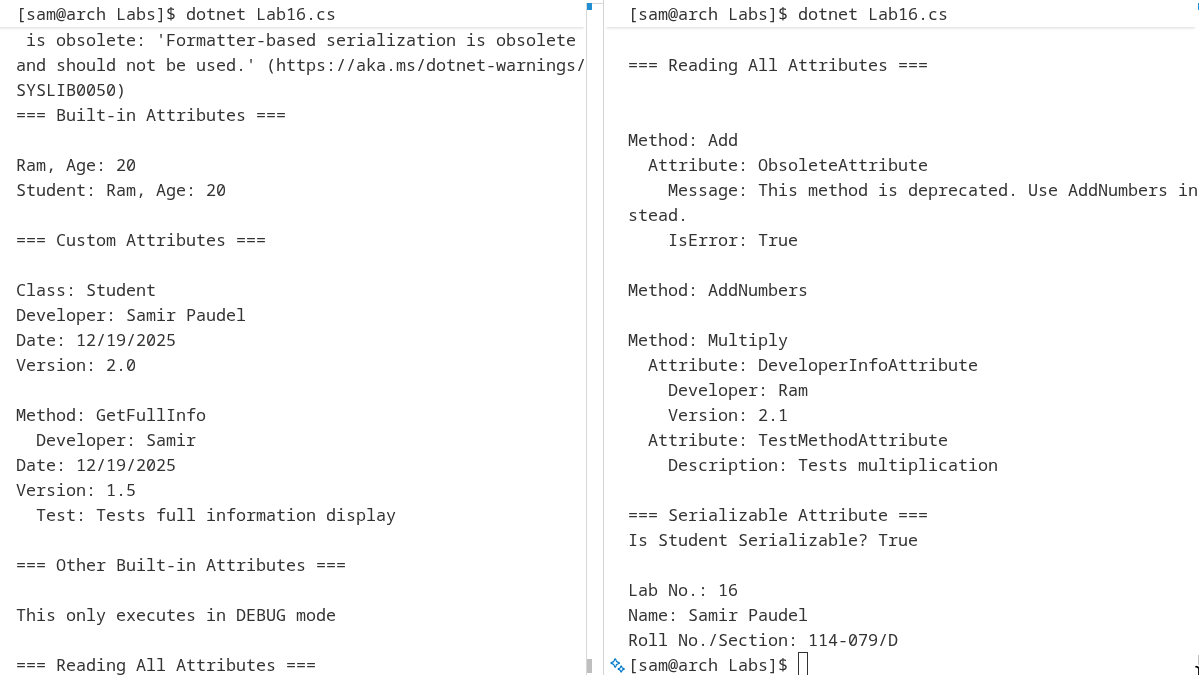
\includegraphics[width=0.7\linewidth]{lab16.png}
\end{figure}

\newpage

% ======================== LAB 17 ========================
\section*{Lab 17: Asynchronous Programming}

\subsection*{Title}
WAP to demonstrate asynchronous programming in C\# using async and await keywords.

\subsection*{Theory}
\textbf{Async/Await} enables asynchronous programming without blocking threads. \texttt{async} methods return \texttt{Task} or \texttt{Task<T>}. \texttt{await} pauses execution until task completes.

\texttt{Task.WhenAll} waits for all tasks to complete. \texttt{Task.WhenAny} waits for first completion. Async improves application responsiveness and scalability.

Best for I/O operations, network calls, file operations. Doesn't create new threads - uses task scheduler efficiently.

\subsection*{Code}
\begin{multicols}{2}
\begin{lstlisting}
using System;
using System.Threading;
using System.Threading.Tasks;
using System.Net.Http;

class Program
{
  static async Task Main(string[] args)
  {
    Console.WriteLine("=== Async/Await Basics ===\n");
    
    Console.WriteLine("Starting async operation...");
    await PerformAsyncOperation();
    Console.WriteLine("Async operation completed!\n");
    
    Console.WriteLine("=== Multiple Async Tasks ===\n");
    await RunMultipleTasks();
    
    Console.WriteLine("\n=== Async with Return Value ===\n");
    int result = await CalculateAsync(10, 5);
    Console.WriteLine($"Calculation result: {result}");
    
    Console.WriteLine("\n=== Parallel Async Tasks ===\n");
    await RunParallelTasks();
    
    Console.WriteLine("\n=== Exception Handling in Async ===\n");
    await HandleAsyncException();
    
    Console.WriteLine("\n=== Task.WhenAll ===\n");
    await DemoTaskWhenAll();
    
    Console.WriteLine("\n=== Task.WhenAny ===\n");
    await DemoTaskWhenAny();
    
    Console.WriteLine("\nLab No.: 17");
    Console.WriteLine("Name: Samir Paudel");
    Console.WriteLine("Roll No./Section: 114-079/D");
  }
  
  static async Task PerformAsyncOperation()
  {
    Console.WriteLine("  Task started...");
    await Task.Delay(2000); // Simulate 2 second delay
    Console.WriteLine("  Task completed after 2 seconds");
  }
  
  static async Task RunMultipleTasks()
  {
    Console.WriteLine("Task 1 starting...");
    await Task1();
    
    Console.WriteLine("Task 2 starting...");
    await Task2();
    
    Console.WriteLine("Both tasks completed");
  }
  
  static async Task Task1()
  {
    await Task.Delay(1000);
    Console.WriteLine("  Task 1 done (1 sec)");
  }
  
  static async Task Task2()
  {
    await Task.Delay(1500);
    Console.WriteLine("  Task 2 done (1.5 sec)");
  }
  
  static async Task<int> CalculateAsync(int a, int b)
  {
    Console.WriteLine($"Calculating {a} + {b}...");
    await Task.Delay(1000);
    return a + b;
  }
  
  static async Task RunParallelTasks()
  {
    Console.WriteLine("Starting 3 tasks in parallel...");
    
    var task1 = DownloadDataAsync("File1", 1000);
    var task2 = DownloadDataAsync("File2", 1500);
    var task3 = DownloadDataAsync("File3", 2000);
    
    await Task.WhenAll(task1, task2, task3);
    
    Console.WriteLine("\nAll downloads completed!");
    Console.WriteLine($"Total time: ~2 seconds (parallel execution)");
  }
  
  static async Task DownloadDataAsync(string fileName, int delay)
  {
    Console.WriteLine($"  Downloading {fileName}...");
    await Task.Delay(delay);
    Console.WriteLine($"  {fileName} downloaded ({delay}ms)");
  }
  
  static async Task HandleAsyncException()
  {
    try
    {
      await TaskThatThrowsException();
    }
    catch (Exception ex)
    {
      Console.WriteLine($"Caught exception: {ex.Message}");
    }
  }
  
  static async Task TaskThatThrowsException()
  {
    await Task.Delay(500);
    throw new Exception("Something went wrong in async task!");
  }
  
  static async Task DemoTaskWhenAll()
  {
    var tasks = new[]
    {
      ProcessDataAsync("Data1", 1000),
      ProcessDataAsync("Data2", 1500),
      ProcessDataAsync("Data3", 800)
    };
    
    Console.WriteLine("Waiting for all tasks...");
    var results = await Task.WhenAll(tasks);
    
    Console.WriteLine("\nAll results:");
    foreach (var result in results)
      Console.WriteLine($"  {result}");
  }
  
  static async Task<string> ProcessDataAsync(string data, int delay)
  {
    await Task.Delay(delay);
    return $"{data} processed in {delay}ms";
  }
  
  static async Task DemoTaskWhenAny()
  {
    var task1 = DelayedTaskAsync("Fast Task", 1000);
    var task2 = DelayedTaskAsync("Medium Task", 2000);
    var task3 = DelayedTaskAsync("Slow Task", 3000);
    
    Console.WriteLine("Waiting for first task to complete...");
    
    var completedTask = await Task.WhenAny(task1, task2, task3);
    var result = await completedTask;
    
    Console.WriteLine($"\nFirst completed: {result}");
    Console.WriteLine("Other tasks still running in background");
  }
  
  static async Task<string> DelayedTaskAsync(string name, int delay)
  {
    Console.WriteLine($"  {name} started");
    await Task.Delay(delay);
    Console.WriteLine($"  {name} completed");
    return name;
  }
}
\end{lstlisting}
\end{multicols}

\subsection*{Output}
\begin{figure}[h!]
    \raggedright
    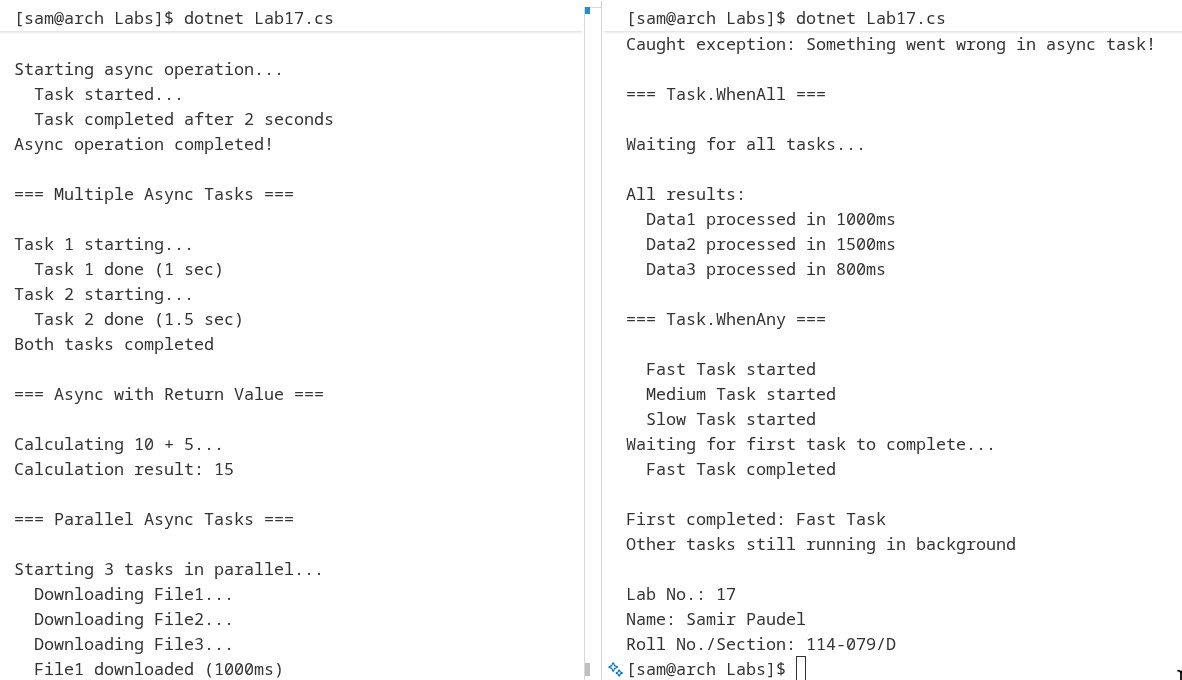
\includegraphics[width=0.7\linewidth]{lab17.png}
\end{figure}

\newpage

% 
% ======================== LAB 18 ========================
\section*{Lab 18: ASP.NET Core MVC Application}

\subsection*{Title}
Create an ASP.Net Core MVC project (WebApp1BySamir) with Razor pages, Model validation, and CRUD forms.

\subsection*{Theory}
ASP.NET Core MVC follows Model-View-Controller pattern. Models represent data with validation attributes. Views (Razor pages) display UI. Controllers handle HTTP requests and return responses. Tag Helpers simplify form creation. Server-side validation ensures data integrity before processing.

\subsection*{Project Structure}
\begin{verbatim}
WebApp1BySamir/
├── Controllers/
│   └── MyController.cs
├── Models/
│   └── Student.cs
└── Views/
    └── My/
        ├── MyRazorPage.cshtml
        ├── CreateStudent.cshtml
        └── StudentDetails.cshtml
\end{verbatim}

\subsection*{Key Code}

\textbf{Student Model with Validation:}
\begin{lstlisting}[basicstyle=\ttfamily\tiny]
public class Student
{
    [Required(ErrorMessage = "Student ID is required")]
    [Range(1, 9999, ErrorMessage = "ID must be between 1 and 9999")]
    public int StdID { get; set; }

    [Required, StringLength(100, MinimumLength = 2)]
    public string Name { get; set; }

    [Required, EmailAddress]
    public string Email { get; set; }
}
\end{lstlisting}

\textbf{Controller Actions:}
\begin{lstlisting}[basicstyle=\ttfamily\tiny]
[HttpPost]
public IActionResult CreateStudent(Student student)
{
    if (ModelState.IsValid)
        return RedirectToAction("StudentDetails", student);
    return View(student);
}
\end{lstlisting}

\subsection*{Features}
\begin{itemize}
    \item MyRazorPage: Displays current date/time, name (Samir Paudel), roll no (114-079/D), multiplication table of 80
    \item Create Student form with validation (Name, Email, Age, Faculty, etc.)
    \item Server-side validation with error messages in red
    \item Redirect to StudentDetails page on successful submission
    \item Navbar links: "MyRazorPage" and "Create Student Record"
\end{itemize}

\subsection*{Output}
\begin{figure}[h!]
    \centering
    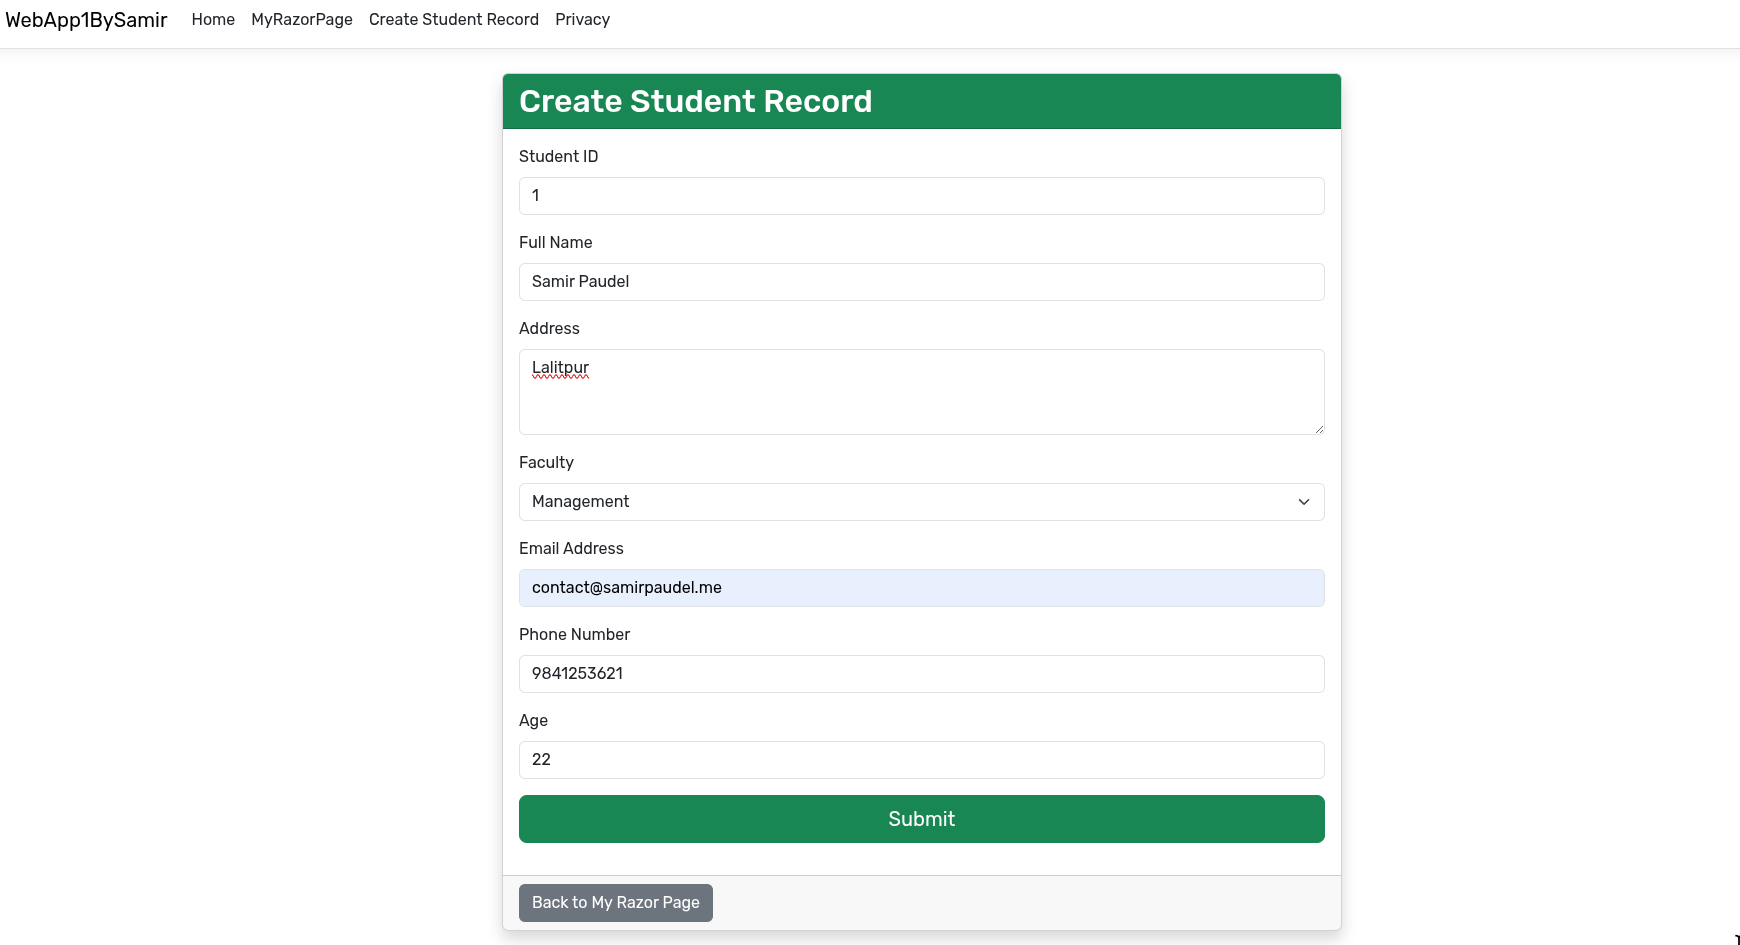
\includegraphics[width=0.45\textwidth]{lab18.1.png}
    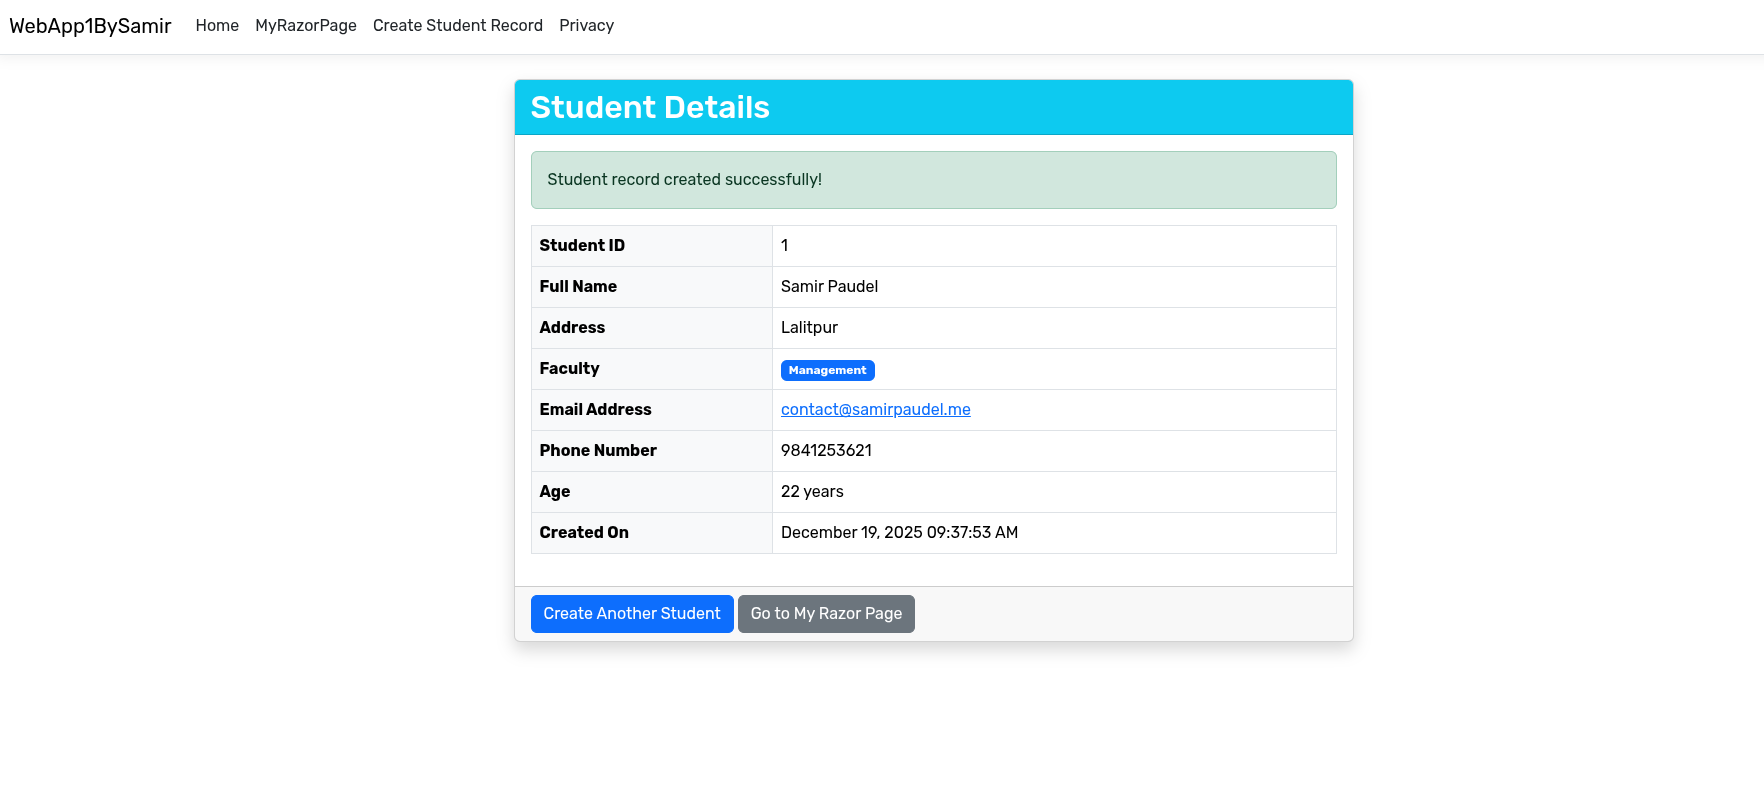
\includegraphics[width=0.45\textwidth]{lab18.2.png}
    \caption*{Student form validation and details}
\end{figure}

\newpage

% ======================== LAB 19 ========================
\section*{Lab 19: Dependency Injection in ASP.NET Core}

\subsection*{Title}
Create a project (WebApp2BySamir) to illustrate dependency injection with different service lifetimes.

\subsection*{Theory}
Dependency Injection is a design pattern where objects receive dependencies from external sources. ASP.NET Core has built-in DI container with three service lifetimes: \textbf{Transient} (new instance every time), \textbf{Scoped} (one instance per request), \textbf{Singleton} (single instance for app lifetime).

\subsection*{Service Registration (Program.cs)}
\begin{lstlisting}[basicstyle=\ttfamily\scriptsize]
// Transient: New instance every time
builder.Services.AddTransient<ITimeService, TimeService>();

// Scoped: Same instance within a request
builder.Services.AddScoped<ILoggerService, LoggerService>();

// Singleton: Single instance throughout app
builder.Services.AddSingleton<IGreetingService, GreetingService>();
\end{lstlisting}

\subsection*{Constructor Injection}
\begin{lstlisting}[basicstyle=\ttfamily\scriptsize]
public class DIController : Controller
{
    private readonly IGreetingService _greetingService;
    private readonly ITimeService _timeService;

    public DIController(IGreetingService greeting, 
                       ITimeService time)
    {
        _greetingService = greeting;
        _timeService = time;
    }
}
\end{lstlisting}

\subsection*{Services Implemented}
\begin{itemize}
    \item \textbf{IGreetingService} (Singleton): Provides greeting messages
    \item \textbf{IDataService} (Singleton): Manages student list, shows service creation time
    \item \textbf{ILoggerService} (Scoped): Logs activities with instance ID
    \item \textbf{ITimeService} (Transient): Returns current time, demonstrates new instances
\end{itemize}

\subsection*{Output}
\begin{figure}[h!]
    \centering
    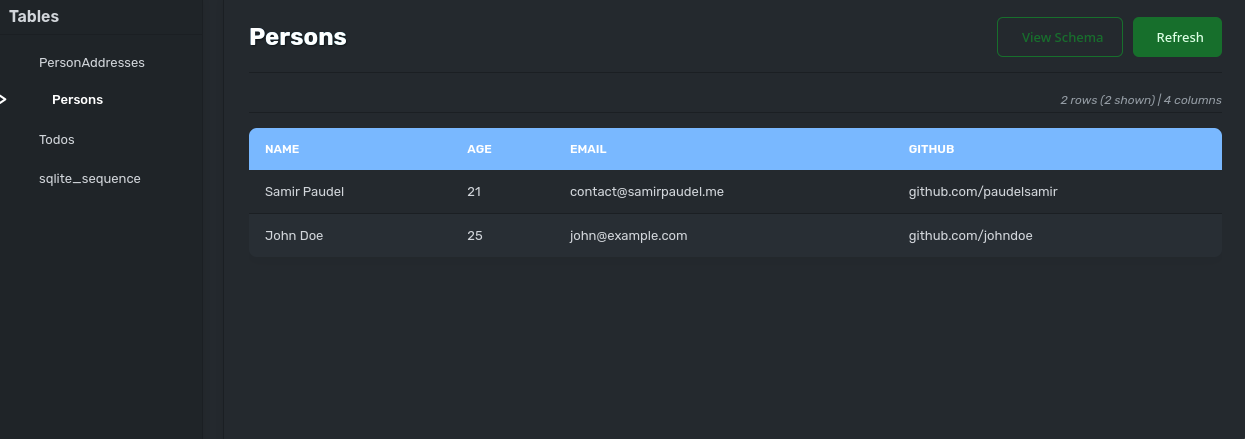
\includegraphics[width=0.9\textwidth]{lab19.png}
    \caption*{Dependency Injection service lifetimes}
\end{figure}

\newpage

% ======================== LAB 20 ========================
\section*{Lab 20: Database CRUD Operations with SQL Server}

\subsection*{Title}
Console application (DatabaseCRUDBySamir) demonstrating INSERT, READ, UPDATE, DELETE operations with SQL Server.

\subsection*{Theory}
CRUD operations are fundamental database operations. ADO.NET provides classes like SqlConnection, SqlCommand, and SqlDataReader for database access. Parameterized queries prevent SQL injection. The application uses try-catch for error handling and using statements for resource disposal.

\subsection*{Database Table Structure}
\begin{lstlisting}[language=SQL, basicstyle=\ttfamily\tiny]
CREATE TABLE Students (
    StudentID INT PRIMARY KEY IDENTITY(1,1),
    Name NVARCHAR(100) NOT NULL,
    Email NVARCHAR(100) NOT NULL,
    Age INT NOT NULL,
    Course NVARCHAR(50) NOT NULL,
    City NVARCHAR(50) NOT NULL,
    CreatedDate DATETIME DEFAULT GETDATE()
);
\end{lstlisting}

\subsection*{CRUD Operations}

\textbf{1. INSERT:}
\begin{lstlisting}[basicstyle=\ttfamily\tiny]
string query = @"INSERT INTO Students (Name, Email, Age, Course, City) 
                VALUES (@Name, @Email, @Age, @Course, @City)";
cmd.Parameters.AddWithValue("@Name", name);
cmd.ExecuteNonQuery();
\end{lstlisting}

\textbf{2. READ:}
\begin{lstlisting}[basicstyle=\ttfamily\tiny]
string query = "SELECT * FROM Students ORDER BY StudentID";
using (SqlDataReader reader = cmd.ExecuteReader())
{
    while (reader.Read())
        Console.WriteLine($"{reader["Name"]} - {reader["Email"]}");
}
\end{lstlisting}

\textbf{3. UPDATE:}
\begin{lstlisting}[basicstyle=\ttfamily\tiny]
string query = @"UPDATE Students SET Name = @Name, Email = @Email 
                WHERE StudentID = @StudentID";
\end{lstlisting}

\textbf{4. DELETE:}
\begin{lstlisting}[basicstyle=\ttfamily\tiny]
string query = "DELETE FROM Students WHERE StudentID = @StudentID";
\end{lstlisting}

\subsection*{Features}
\begin{itemize}
    \item Auto-creates database and table on first run
    \item Menu-driven interface (Insert, Read All, Read by ID, Update, Delete)
    \item Parameterized queries for security
    \item Comprehensive error handling
    \item Display records in formatted table
\end{itemize}

\subsection*{Output}
\begin{figure}[h!]
    \centering
    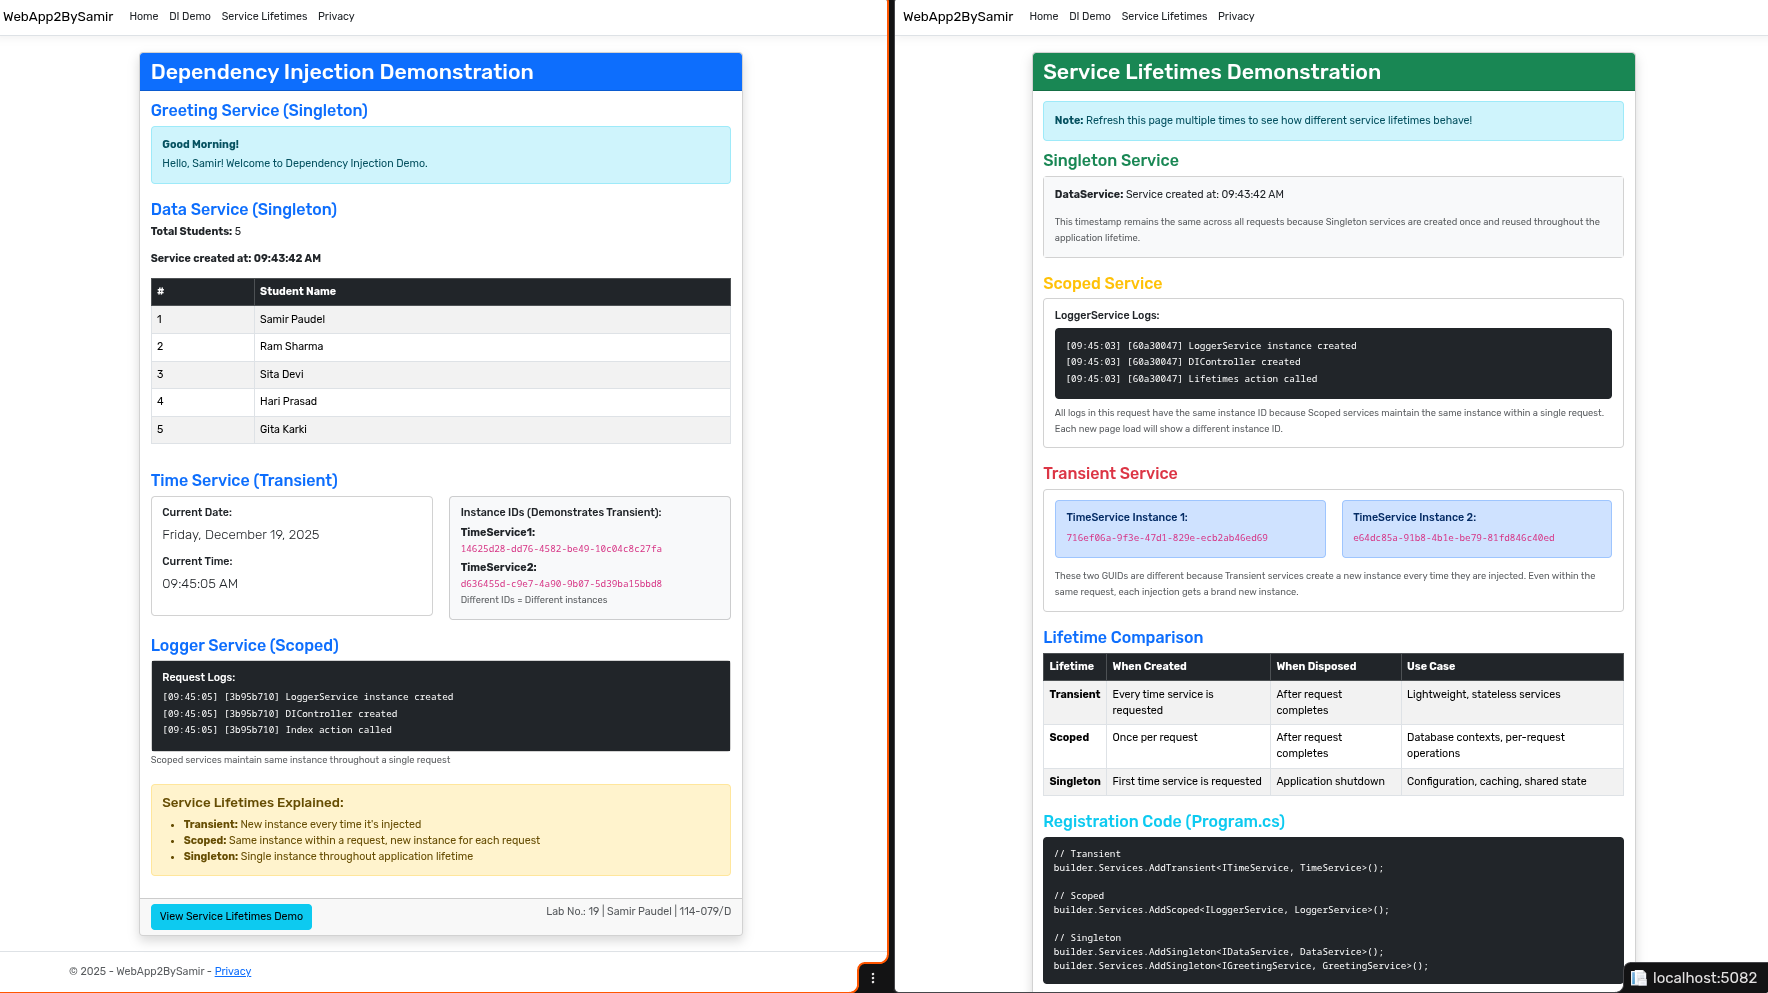
\includegraphics[width=0.9\textwidth]{lab20.png}
    \caption*{Database CRUD operations}
\end{figure}

\newpage

% ======================== LAB 21 ========================
\section*{Lab 21: ASP.NET Core MVC CRUD with ADO.NET}

\subsection*{Title}
Create CRUD application using ASP.NET Core MVC template with ADO.NET (WebApp3BySamir).

\subsection*{Theory}
ADO.NET provides low-level database access in .NET. Uses SqlConnection for database connection, SqlCommand for executing queries, and SqlDataReader for reading data. Parameterized queries prevent SQL injection. This approach gives full control over SQL and database operations.

\subsection*{Database Structure}
\begin{lstlisting}[language=SQL, basicstyle=\ttfamily\tiny]
CREATE TABLE Products (
    ProductID INT PRIMARY KEY IDENTITY(1,1),
    ProductName NVARCHAR(100) NOT NULL,
    Price DECIMAL(18,2) NOT NULL,
    Quantity INT NOT NULL,
    Category NVARCHAR(50),
    CreatedDate DATETIME DEFAULT GETDATE()
);
\end{lstlisting}

\subsection*{Key Components}

\textbf{1. Data Access Layer:}
\begin{lstlisting}[basicstyle=\ttfamily\tiny]
public bool InsertProduct(Product product)
{
    using (SqlConnection conn = new SqlConnection(_connectionString))
    {
        conn.Open();
        string query = @"INSERT INTO Products (ProductName, Price, Quantity, Category, CreatedDate) 
                        VALUES (@ProductName, @Price, @Quantity, @Category, @CreatedDate)";
        using (SqlCommand cmd = new SqlCommand(query, conn))
        {
            cmd.Parameters.AddWithValue("@ProductName", product.ProductName);
            cmd.Parameters.AddWithValue("@Price", product.Price);
            // ... other parameters
            cmd.ExecuteNonQuery();
        }
    }
}
\end{lstlisting}

\textbf{2. Controller Actions:}
\begin{lstlisting}[basicstyle=\ttfamily\tiny]
[HttpPost]
public IActionResult Create(Product product)
{
    if (ModelState.IsValid)
    {
        if (_dataAccess.InsertProduct(product))
            return RedirectToAction(nameof(Index));
    }
    return View(product);
}
\end{lstlisting}

\subsection*{Features}
\begin{itemize}
    \item Product management with full CRUD
    \item Parameterized SQL queries for security
    \item Auto-creates database and table on startup
    \item Model validation with Data Annotations
    \item Bootstrap UI with responsive design
    \item TempData for success/error messages
\end{itemize}

\subsection*{Output}
\begin{figure}[h!]
    \centering
    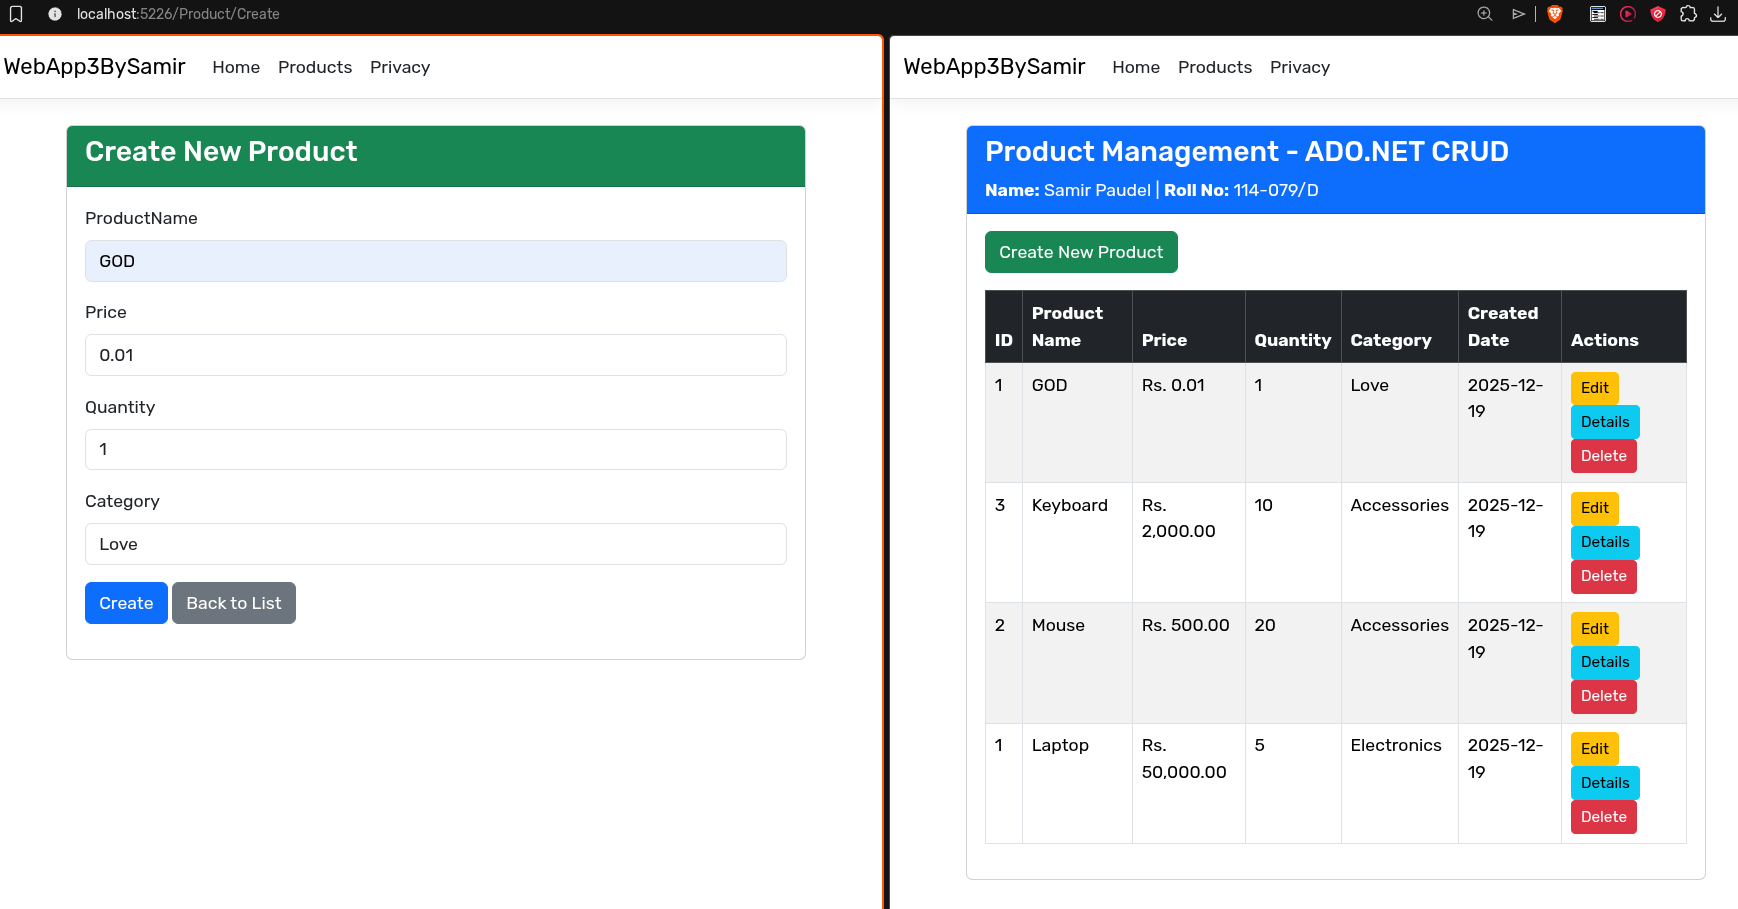
\includegraphics[width=0.9\textwidth]{lab21.png}
    \caption*{MVC CRUD with ADO.NET}
\end{figure}

\newpage

% ======================== LAB 22 ========================
\section*{Lab 22: Entity Framework Core - Code First Approach}

\subsection*{Title}
Create CRUD application using ASP.NET Core MVC with Entity Framework Core Code First (WebApp4BySamir).

\subsection*{Theory}
EF Core Code First creates database from C\# models. DbContext manages entity objects and database connection. Migrations track schema changes. LINQ queries are translated to SQL automatically. Provides change tracking, lazy loading, and relationship management.

\subsection*{Model Definition}
\begin{lstlisting}[basicstyle=\ttfamily\tiny]
public class Book
{
    [Key]
    public int BookId { get; set; }
    
    [Required, StringLength(200)]
    public string Title { get; set; }
    
    [Required, StringLength(100)]
    public string Author { get; set; }
    
    [Range(0.01, 999999.99)]
    public decimal Price { get; set; }
}
\end{lstlisting}

\subsection*{DbContext Configuration}
\begin{lstlisting}[basicstyle=\ttfamily\tiny]
public class ApplicationDbContext : DbContext
{
    public DbSet<Book> Books { get; set; }
    
    protected override void OnModelCreating(ModelBuilder modelBuilder)
    {
        modelBuilder.Entity<Book>().Property(e => e.Price)
            .HasColumnType("decimal(18,2)");
        
        // Seed data
        modelBuilder.Entity<Book>().HasData(
            new Book { BookId = 1, Title = "C# Guide", Author = "Samir" }
        );
    }
}
\end{lstlisting}

\subsection*{Controller with EF Core}
\begin{lstlisting}[basicstyle=\ttfamily\tiny]
public async Task<IActionResult> Index()
{
    return View(await _context.Books.OrderBy(b => b.BookId).ToListAsync());
}

[HttpPost]
public async Task<IActionResult> Create(Book book)
{
    if (ModelState.IsValid)
    {
        _context.Add(book);
        await _context.SaveChangesAsync();
        return RedirectToAction(nameof(Index));
    }
    return View(book);
}
\end{lstlisting}

\subsection*{Migration Commands}
\begin{verbatim}
dotnet ef migrations add InitialCreate
dotnet ef database update
\end{verbatim}

\subsection*{Features}
\begin{itemize}
    \item Entity Framework Core with async operations
    \item Auto-migration on application startup
    \item LINQ queries (OrderBy, Where, FirstOrDefault)
    \item DbContext dependency injection
    \item Seed data for initial records
    \item Book management CRUD operations
\end{itemize}

\subsection*{Output}
\begin{figure}[h!]
    \centering
    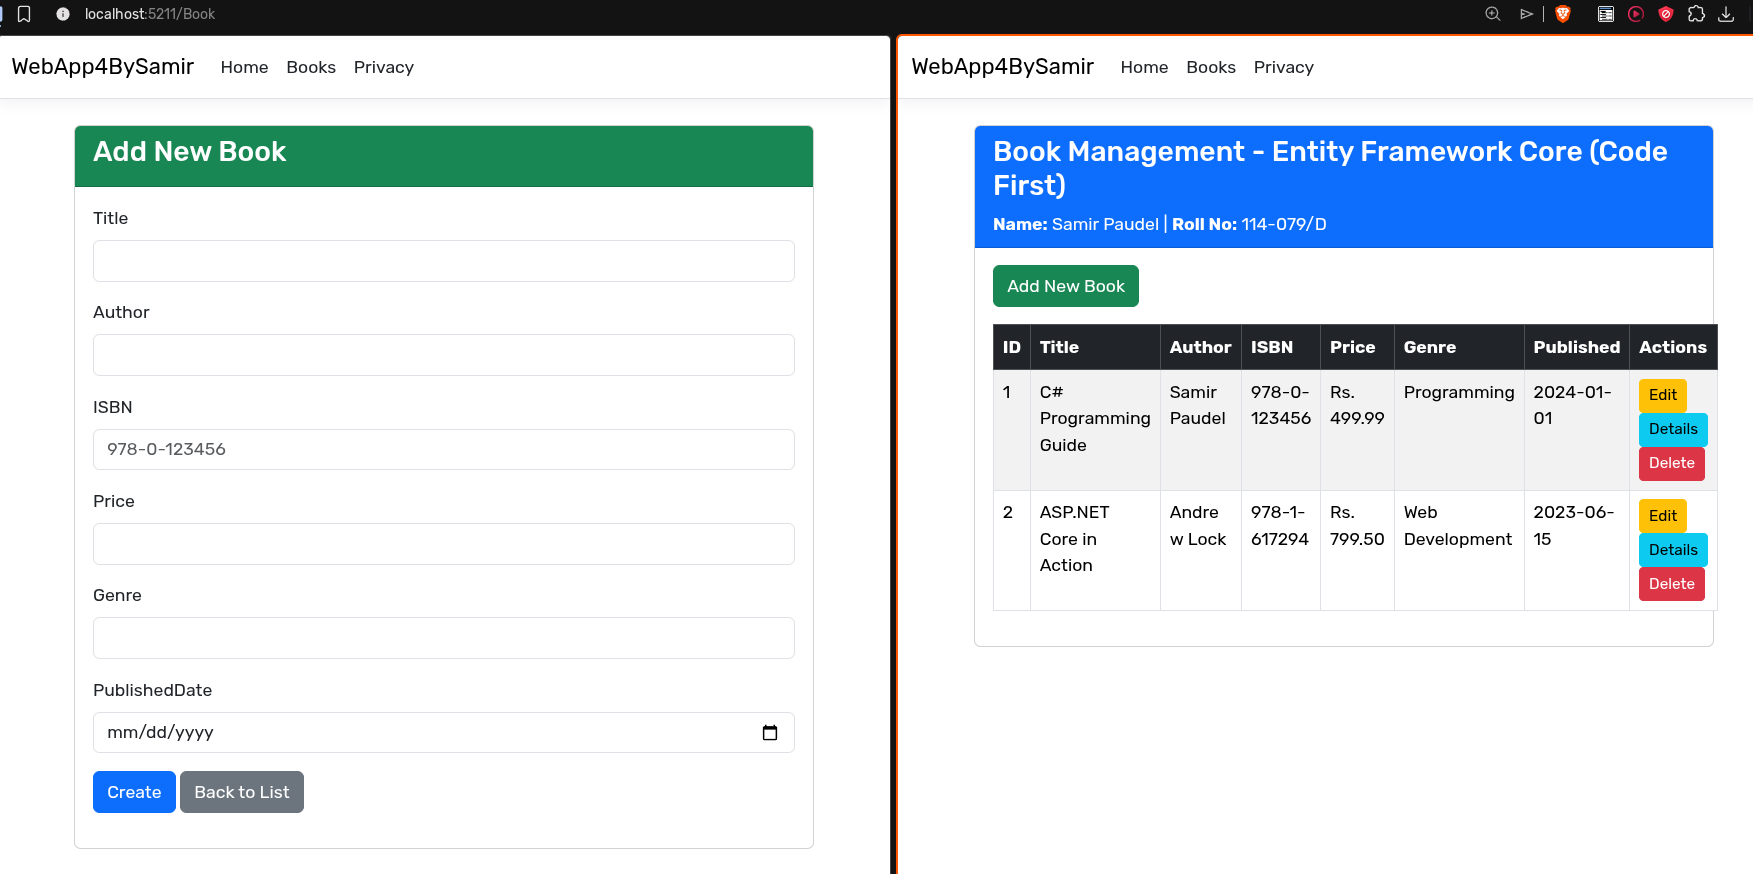
\includegraphics[width=0.9\textwidth]{lab22.png}
    \caption*{EF Core Code First}
\end{figure}

\newpage

% ======================== LAB 23 ========================
\section*{Lab 23: Entity Framework Core - Database First Approach}

\subsection*{Title}
Create ASP.NET Core application demonstrating EF Core Database First (WebApp5BySamir).

\subsection*{Theory}
Database First starts with existing database and generates models. Uses scaffolding (reverse engineering) to create entity classes and DbContext from database schema. Useful for legacy databases or when database design is done separately.

\subsection*{Workflow}
\begin{enumerate}
    \item Create database and tables in SQL Server
    \item Install EF Core tools and SqlServer provider
    \item Run scaffold command to generate models
    \item Use generated DbContext in controllers
\end{enumerate}

\subsection*{Database Creation}
\begin{lstlisting}[language=SQL, basicstyle=\ttfamily\tiny]
CREATE DATABASE WebApp5DB;
USE WebApp5DB;

CREATE TABLE Employees (
    EmployeeID INT PRIMARY KEY IDENTITY(1,1),
    FirstName NVARCHAR(50) NOT NULL,
    LastName NVARCHAR(50) NOT NULL,
    Email NVARCHAR(100),
    Department NVARCHAR(50),
    Salary DECIMAL(18,2),
    HireDate DATETIME DEFAULT GETDATE()
);
\end{lstlisting}

\subsection*{Scaffold Command}
\begin{lstlisting}[basicstyle=\ttfamily\scriptsize]
dotnet ef dbcontext scaffold 
  "Server=localhost;Database=WebApp5DB;Trusted_Connection=True;" 
  Microsoft.EntityFrameworkCore.SqlServer 
  --output-dir Models 
  --context EmployeeDbContext
\end{lstlisting}

This generates:
\begin{itemize}
    \item \texttt{Employee.cs} - Model with properties matching table columns
    \item \texttt{EmployeeDbContext.cs} - DbContext with DbSet and configurations
\end{itemize}

\subsection*{Generated Model Example}
\begin{lstlisting}[basicstyle=\ttfamily\tiny]
public partial class Employee
{
    public int EmployeeId { get; set; }
    public string FirstName { get; set; }
    public string LastName { get; set; }
    public string? Email { get; set; }
    public decimal? Salary { get; set; }
    public DateTime? HireDate { get; set; }
}
\end{lstlisting}

\subsection*{Usage in Controller}
\begin{lstlisting}[basicstyle=\ttfamily\tiny]
public class EmployeeController : Controller
{
    private readonly EmployeeDbContext _context;
    
    public async Task<IActionResult> Index() 
        => View(await _context.Employees.ToListAsync());
}
\end{lstlisting}

\subsection*{Advantages vs Code First}
\begin{itemize}
    \item Works with existing/legacy databases
    \item No manual model creation needed
    \item Database schema is source of truth
    \item Perfect for DBA-controlled environments
\end{itemize}

\subsection*{Output}
[Screenshots: SQL Server database with Employees table, Scaffolded files in project, Employee list view, Generated DbContext code]

\newpage

% ======================== LAB 24 ========================
\section*{Lab 24: ASP.NET Core Web API with Swagger}

\subsection*{Title}
Create Web API using ASP.NET Core and Entity Framework Core with Postman and Swagger testing (WebApiBySamir).

\subsection*{Theory}
Web APIs provide HTTP endpoints for client applications. RESTful design uses HTTP verbs (GET, POST, PUT, DELETE). Swagger/OpenAPI generates interactive API documentation. Returns JSON/XML data instead of HTML views.

\subsection*{API Controller}
\begin{lstlisting}[basicstyle=\ttfamily\tiny]
[Route("api/[controller]")]
[ApiController]
public class TasksController : ControllerBase
{
    private readonly TaskDbContext _context;
    
    // GET: api/Tasks
    [HttpGet]
    public async Task<ActionResult<IEnumerable<Task>>> GetTasks()
        => await _context.Tasks.ToListAsync();
    
    // POST: api/Tasks
    [HttpPost]
    public async Task<ActionResult<Task>> PostTask(Task task)
    {
        _context.Tasks.Add(task);
        await _context.SaveChangesAsync();
        return CreatedAtAction(nameof(GetTask), new { id = task.TaskId }, task);
    }
    
    // PUT: api/Tasks/5
    [HttpPut("{id}")]
    public async Task<IActionResult> PutTask(int id, Task task)
    {
        _context.Entry(task).State = EntityState.Modified;
        await _context.SaveChangesAsync();
        return NoContent();
    }
}
\end{lstlisting}

\subsection*{Swagger Configuration (Program.cs)}
\begin{lstlisting}[basicstyle=\ttfamily\tiny]
builder.Services.AddSwaggerGen(c =>
{
    c.SwaggerDoc("v1", new OpenApiInfo
    {
        Title = "Task API by Samir Paudel",
        Version = "v1"
    });
});

app.UseSwagger();
app.UseSwaggerUI(c =>
{
    c.SwaggerEndpoint("/swagger/v1/swagger.json", "Task API v1");
    c.RoutePrefix = string.Empty; // Swagger UI at root
});
\end{lstlisting}

\subsection*{Testing Methods}

\textbf{Swagger UI:}
\begin{itemize}
    \item Navigate to \texttt{https://localhost:5001}
    \item Click "Try it out" on any endpoint
    \item Enter parameters, click "Execute"
    \item View response body and status code
\end{itemize}

\textbf{Postman Testing:}
\begin{lstlisting}[basicstyle=\ttfamily\scriptsize]
GET https://localhost:5001/api/tasks

POST https://localhost:5001/api/tasks
Body (JSON):
{
  "title": "Complete Lab 24",
  "priority": "High",
  "isCompleted": false
}

PUT https://localhost:5001/api/tasks/1
DELETE https://localhost:5001/api/tasks/1
\end{lstlisting}

\subsection*{HTTP Status Codes Used}
\begin{itemize}
    \item 200 OK - Successful GET
    \item 201 Created - Successful POST
    \item 204 No Content - Successful PUT/DELETE
    \item 400 Bad Request - Validation errors
    \item 404 Not Found - Resource doesn't exist
\end{itemize}

\subsection*{Output}
\begin{figure}[h!]
    \centering
    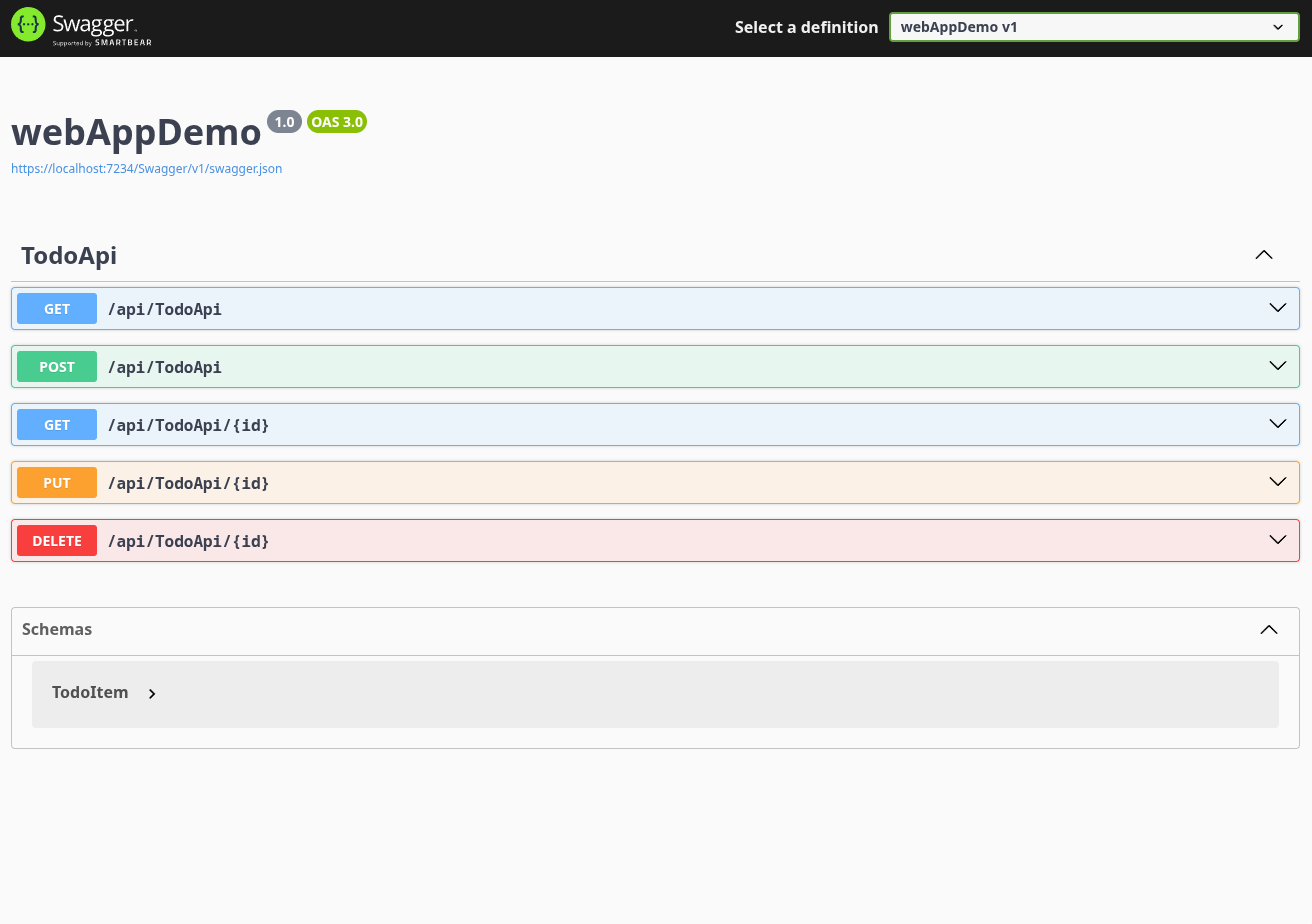
\includegraphics[width=0.9\textwidth]{lab24_swagger.png}
    \caption*{Web API with Swagger}
\end{figure}

\newpage

% ======================== LAB 25 ========================
\section*{Lab 25: State Management in ASP.NET Core}

\subsection*{Title}
Demonstrate state management using Session, HttpContext, TempData, Cookies, Query Strings, and Hidden Fields (WebApp6BySamir).

\subsection*{Theory}
State management preserves data across HTTP requests. Server-side (Session, TempData) stores data on server. Client-side (Cookies, Query Strings, Hidden Fields) stores on client. Each has different scope, lifetime, and use cases.

\subsection*{Implementation}

\textbf{1. Session State:}
\begin{lstlisting}[basicstyle=\ttfamily\tiny]
// Configure in Program.cs
builder.Services.AddDistributedMemoryCache();
builder.Services.AddSession(options => {
    options.IdleTimeout = TimeSpan.FromMinutes(30);
});
app.UseSession();

// Usage
HttpContext.Session.SetString("Username", "Samir Paudel");
var username = HttpContext.Session.GetString("Username");
\end{lstlisting}

\textbf{2. HttpContext.Items:}
\begin{lstlisting}[basicstyle=\ttfamily\tiny]
HttpContext.Items["RequestTime"] = DateTime.Now;
var time = HttpContext.Items["RequestTime"];
\end{lstlisting}

\textbf{3. TempData:}
\begin{lstlisting}[basicstyle=\ttfamily\tiny]
TempData["SuccessMessage"] = "Data saved!";
var msg = TempData["SuccessMessage"]; // Auto-deleted after read
TempData.Keep("SuccessMessage"); // Keep for next request
\end{lstlisting}

\textbf{4. Cookies:}
\begin{lstlisting}[basicstyle=\ttfamily\tiny]
Response.Cookies.Append("Theme", "Dark", new CookieOptions
{
    Expires = DateTimeOffset.Now.AddDays(7),
    HttpOnly = true
});
Request.Cookies.TryGetValue("Theme", out string theme);
\end{lstlisting}

\textbf{5. Query Strings:}
\begin{lstlisting}[basicstyle=\ttfamily\tiny]
// In view: <a href="/Product/Details?id=5&name=Laptop">
public IActionResult Details(int id, string name) { }
\end{lstlisting}

\textbf{6. Hidden Fields:}
\begin{lstlisting}[basicstyle=\ttfamily\tiny]
<input type="hidden" name="ProductId" value="@Model.ProductId" />
\end{lstlisting}

\subsection*{Comparison}
\begin{tabular}{|l|l|l|l|}
\hline
\textbf{Technique} & \textbf{Storage} & \textbf{Lifetime} & \textbf{Use Case} \\
\hline
Session & Server & Until timeout & User auth, cart \\
HttpContext.Items & Server & Single request & Middleware data \\
TempData & Server & One redirect & Flash messages \\
Cookies & Client & Set expiration & Preferences \\
Query String & Client & Single request & Filtering \\
Hidden Field & Client & Form post & CSRF tokens \\
\hline
\end{tabular}

\subsection*{Output}
\begin{figure}[h!]
    \centering
    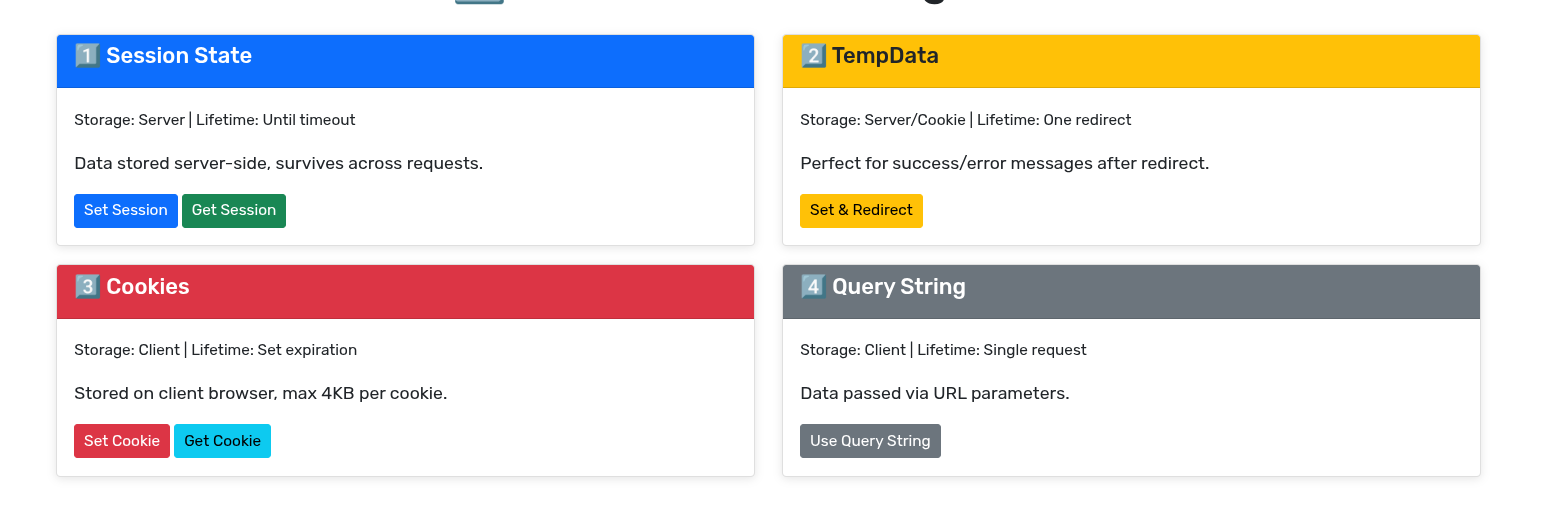
\includegraphics[width=0.9\textwidth]{lab25.png}
    \caption*{State Management techniques}
\end{figure}

\newpage

% ======================== LAB 26 ========================
\section*{Lab 26: Client-Side Development}

\subsection*{Part A: jQuery Form Validation}

\textbf{Overview:} Signup form with client-side validation using jQuery. Display name and roll at top.

\textbf{Key Features:}
\begin{itemize}
    \item Real-time validation on blur event
    \item Regex patterns for email and phone
    \item Password confirmation matching
    \item Error messages below fields (red color)
    \item Success message on valid submission
\end{itemize}

\textbf{Validation Example:}
\begin{lstlisting}[language=JavaScript, basicstyle=\ttfamily\tiny]
function validateEmail() {
    let email = $('#email').val().trim();
    let regex = /^[a-zA-Z0-9._-]+@[a-zA-Z0-9.-]+\.[a-zA-Z]{2,6}$/;
    if (!regex.test(email)) {
        $('#email-error').show();
        return false;
    }
    $('#email-error').hide();
    return true;
}

$('#signupForm').submit(function(e) {
    e.preventDefault();
    if (validateEmail() && validatePassword()) {
        $('#success-message').text('Signup successful!');
    }
});
\end{lstlisting}

\subsection*{Part B: Angular Calculator App}

\textbf{Project:} AngularAppBySamir

\textbf{Components:}
\begin{itemize}
    \item Navbar with Home and Calculator menus
    \item Footer with copyright and current year
    \item Home page with profile photo
    \item Calculator with two inputs, dropdown, compute button
\end{itemize}

\textbf{Calculator Component:}
\begin{lstlisting}[language=JavaScript, basicstyle=\ttfamily\tiny]
export class CalculatorComponent {
  number1: number = 0;
  number2: number = 0;
  operation: string = 'add';
  result: number | null = null;

  compute(): void {
    switch(this.operation) {
      case 'add': this.result = this.number1 + this.number2; break;
      case 'subtract': this.result = this.number1 - this.number2; break;
      case 'multiply': this.result = this.number1 * this.number2; break;
    }
  }
}
\end{lstlisting}

\textbf{Two-way Binding:}
\begin{lstlisting}[language=HTML, basicstyle=\ttfamily\tiny]
<input type="number" [(ngModel)]="number1">
<select [(ngModel)]="operation">
  <option value="add">Add</option>
  <option value="subtract">Subtract</option>
  <option value="multiply">Multiply</option>
</select>
<button (click)="compute()">Compute</button>
<h3 *ngIf="result !== null">Result: {{ result }}</h3>
\end{lstlisting}

\subsection*{Part C: React Calculator App}

\textbf{Project:} ReactAppBySamir

\textbf{React Hooks Implementation:}
\begin{lstlisting}[language=JavaScript, basicstyle=\ttfamily\tiny]
function Calculator() {
  const [number1, setNumber1] = useState(0);
  const [number2, setNumber2] = useState(0);
  const [operation, setOperation] = useState('add');
  const [result, setResult] = useState(null);

  const compute = () => {
    let calcResult;
    switch(operation) {
      case 'add': calcResult = number1 + number2; break;
      case 'subtract': calcResult = number1 - number2; break;
      case 'multiply': calcResult = number1 * number2; break;
    }
    setResult(calcResult);
  };

  return (
    <div>
      <input value={number1} onChange={(e) => setNumber1(e.target.value)} />
      <button onClick={compute}>Compute</button>
      {result !== null && <h3>Result: {result}</h3>}
    </div>
  );
}
\end{lstlisting}

\subsection*{Output}
\begin{figure}[h!]
    \centering
    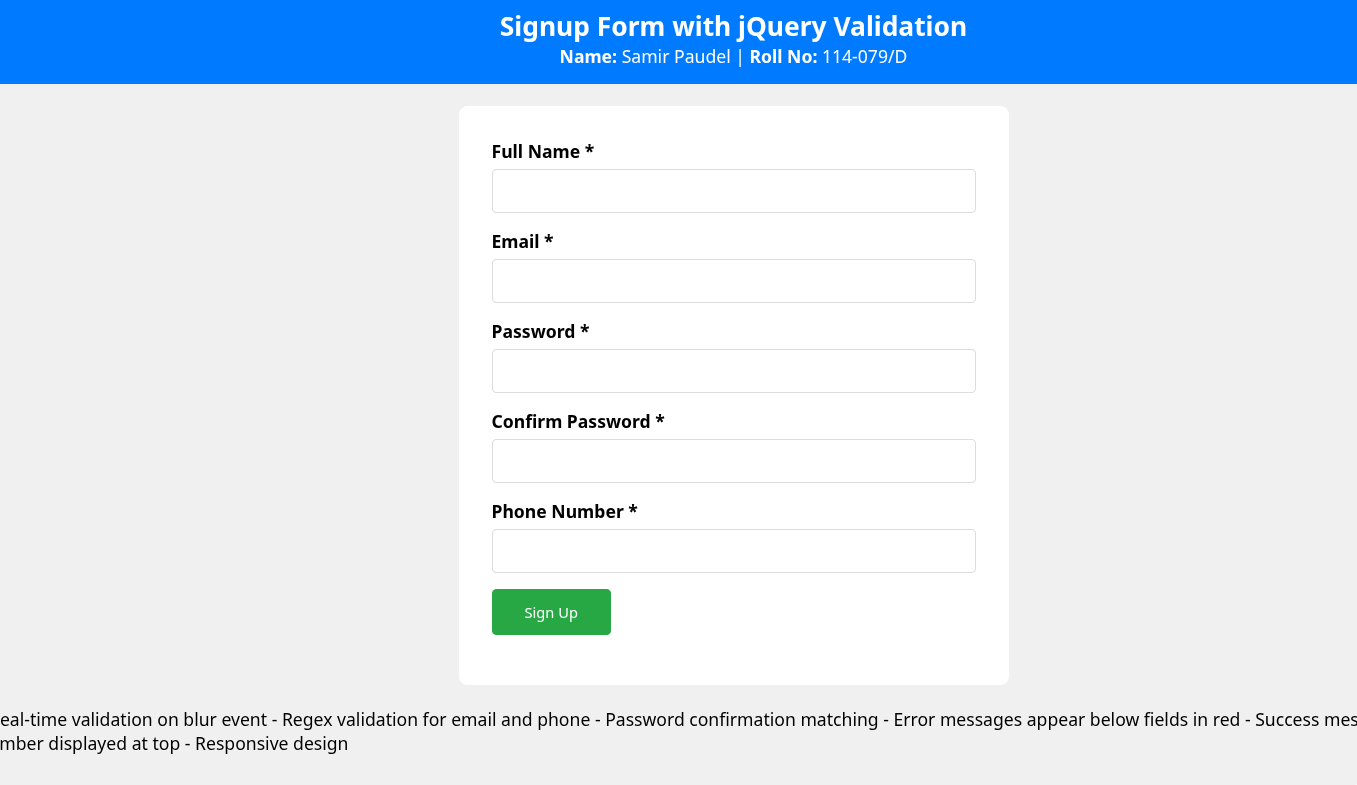
\includegraphics[width=0.45\textwidth]{lab26_jquery.png}
    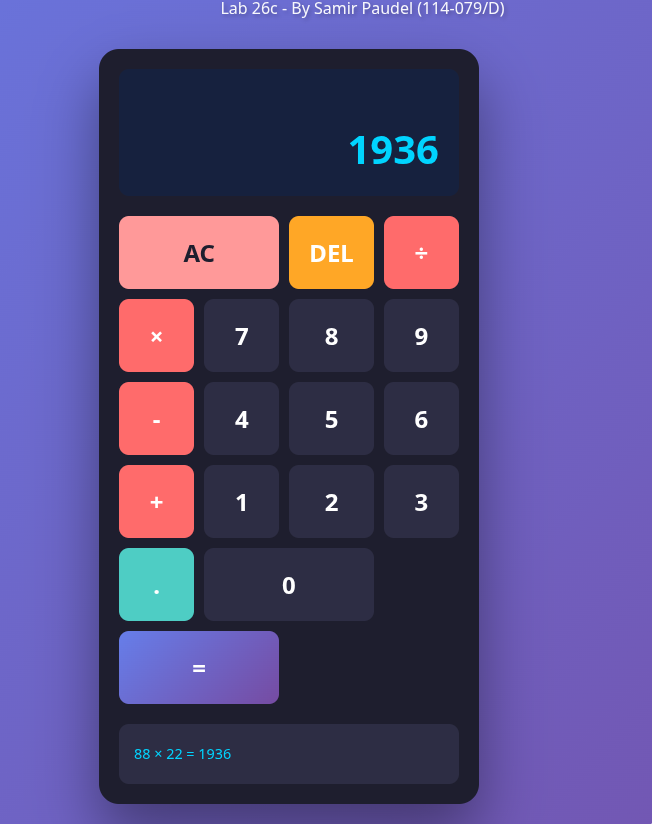
\includegraphics[width=0.45\textwidth]{lab26_react_calculator.png}
    \caption*{jQuery validation and React calculator}
\end{figure}

\newpage

% ======================== LAB 27 ========================
\section*{Lab 27: Authentication \& Authorization}

\subsection*{Title}
Create ASP.NET Core application demonstrating authentication and authorization (WebApp7BySamir).

\subsection*{Theory}
\textbf{Authentication:} Verifies WHO the user is (Login/Register).
\textbf{Authorization:} Determines WHAT the user can access (Roles/Policies).
ASP.NET Core Identity provides user management, password hashing, role management, and claims-based security.

\subsection*{Configuration}
\begin{lstlisting}[basicstyle=\ttfamily\tiny]
// Program.cs
builder.Services.AddIdentity<ApplicationUser, IdentityRole>(options =>
{
    options.Password.RequiredLength = 6;
    options.Password.RequireDigit = true;
})
.AddEntityFrameworkStores<ApplicationDbContext>();

builder.Services.AddAuthorization(options =>
{
    options.AddPolicy("AdminOnly", policy => policy.RequireRole("Admin"));
});
\end{lstlisting}

\subsection*{User Registration}
\begin{lstlisting}[basicstyle=\ttfamily\tiny]
[HttpPost]
public async Task<IActionResult> Register(RegisterViewModel model)
{
    var user = new ApplicationUser
    {
        UserName = model.Email,
        Email = model.Email,
        FullName = model.FullName
    };
    
    var result = await _userManager.CreateAsync(user, model.Password);
    
    if (result.Succeeded)
    {
        await _userManager.AddToRoleAsync(user, "Student");
        await _signInManager.SignInAsync(user, isPersistent: false);
        return RedirectToAction("Index", "Home");
    }
    return View(model);
}
\end{lstlisting}

\subsection*{Login}
\begin{lstlisting}[basicstyle=\ttfamily\tiny]
var result = await _signInManager.PasswordSignInAsync(
    model.Email, model.Password, model.RememberMe, lockoutOnFailure: false);
\end{lstlisting}

\subsection*{Authorization Attributes}
\begin{lstlisting}[basicstyle=\ttfamily\tiny]
[Authorize] // Requires login
public class DashboardController : Controller { }

[Authorize(Roles = "Admin")] // Requires Admin role
public class AdminController : Controller { }

[Authorize(Policy = "AdminOnly")] // Requires policy
public IActionResult ManageUsers() { }
\end{lstlisting}

\subsection*{Check in Views}
\begin{lstlisting}[basicstyle=\ttfamily\tiny]
@if (User.Identity.IsAuthenticated)
{
    <p>Welcome, @User.Identity.Name!</p>
}

@if (User.IsInRole("Admin"))
{
    <a asp-controller="Admin">Admin Panel</a>
}
\end{lstlisting}

\subsection*{Seed Roles}
\begin{lstlisting}[basicstyle=\ttfamily\tiny]
string[] roles = { "Admin", "Teacher", "Student" };
foreach (var role in roles)
{
    if (!await _roleManager.RoleExistsAsync(role))
        await _roleManager.CreateAsync(new IdentityRole(role));
}
\end{lstlisting}

\subsection*{Features}
\begin{itemize}
    \item User registration with password hashing
    \item Login with cookie authentication
    \item Role-based authorization (Admin, Teacher, Student)
    \item Policy-based authorization
    \item Logout functionality
    \item Access denied page
    \item Identity database tables auto-created
\end{itemize}

\subsection*{Output}
\begin{figure}[h!]
    \centering
    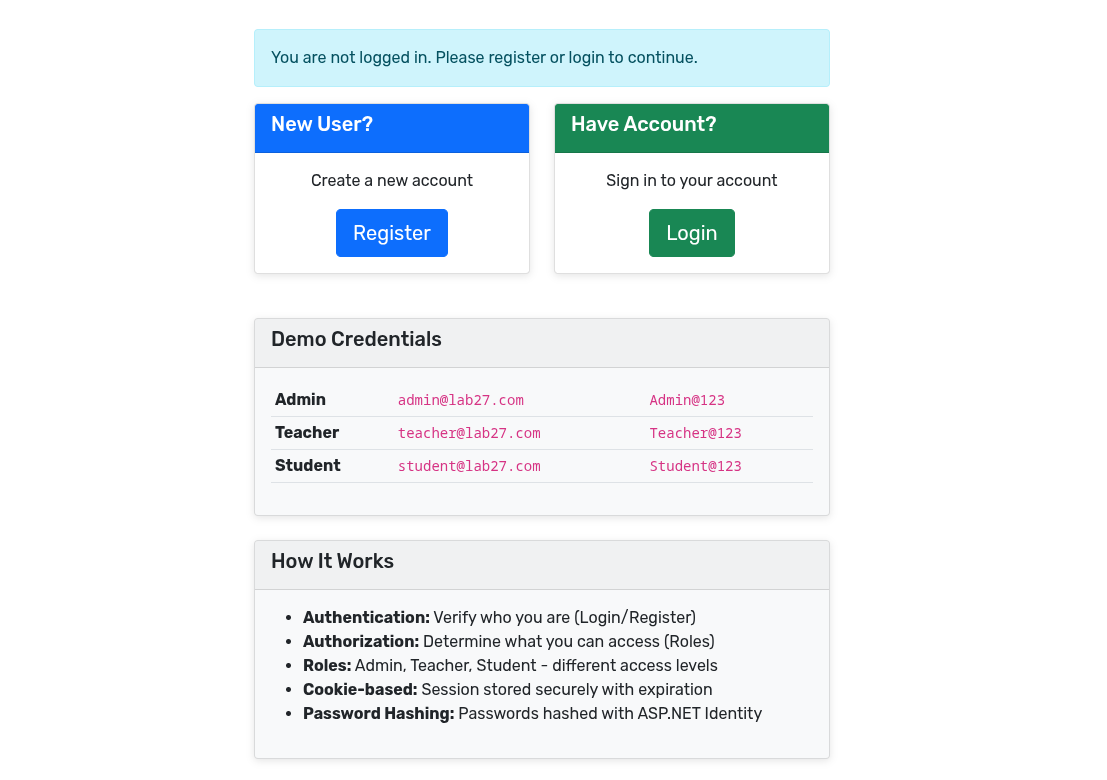
\includegraphics[width=0.9\textwidth]{lab27.png}
    \caption*{Authentication \& Authorization}
\end{figure}

\newpage

% ======================== LAB 28 ========================
\section*{Lab 28: Hosting ASP.NET Core Application}

\subsection*{Title}
Host Lab 23 application (WebApp5BySamir) on free hosting platform with complete documentation.

\subsection*{Hosting Option}

\textbf{ Azure App Service}
\begin{enumerate}
    \item Create Azure account (free tier)
    \item Publish app: \texttt{dotnet publish -c Release}
    \item Create Web App in Azure Portal
    \item Create Azure SQL Database
    \item Deploy via Azure CLI or Visual Studio
    \item Configure connection string in App Settings
\end{enumerate}


\subsection*{Deployment Commands (Azure)}
\begin{lstlisting}[basicstyle=\ttfamily\scriptsize]
# Create resource group
az group create --name WebApp5RG --location eastus

# Create App Service plan
az appservice plan create --name WebApp5Plan --resource-group WebApp5RG --sku F1

# Create web app
az webapp create --name webapp5bysamir --resource-group WebApp5RG --plan WebApp5Plan

# Deploy
az webapp deploy --resource-group WebApp5RG --name webapp5bysamir --src-path ./publish.zip
\end{lstlisting}

\subsection*{Pre-Deployment Checklist}
\begin{itemize}
    \item Set environment to Production
    \item Configure production database connection
    \item Disable detailed errors (use custom error pages)
    \item Enable HTTPS redirection
    \item Test in Release mode locally
    \item Apply all database migrations
    \item Use environment variables for secrets
\end{itemize}

\subsection*{Post-Deployment Verification}
\begin{itemize}
    \item Test all CRUD operations
    \item Verify database connection
    \item Check application logs
    \item Test on mobile/different browsers
    \item Monitor performance
\end{itemize}


\subsection*{Platform Comparison}
\begin{tabular}{|l|l|l|}
\hline
\textbf{Platform} & \textbf{Pros} & \textbf{Database} \\
\hline
Azure & Professional, scalable & SQL Azure \\
Somee & Easy setup & MSSQL included \\
Heroku & Simple deployment & Add-ons \\
Railway & GitHub integration & Multiple options \\
\hline
\end{tabular}

\subsection*{Output}
\begin{figure}[h!]
    \centering
    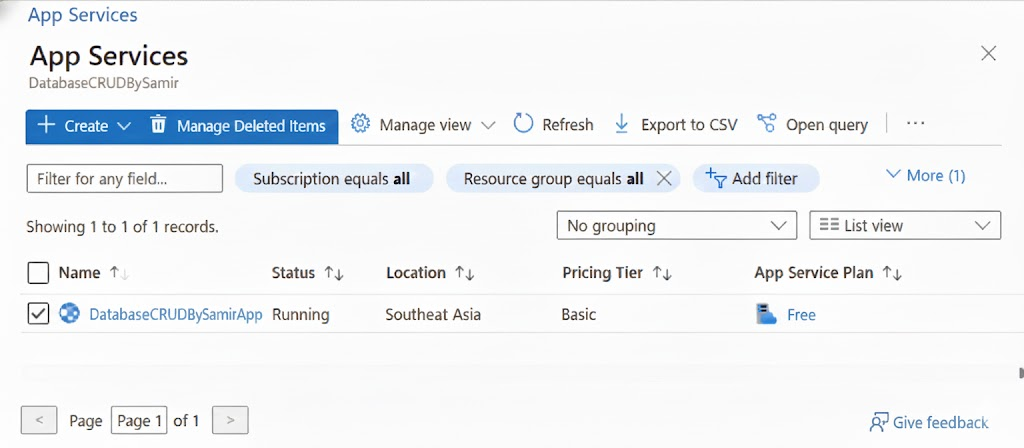
\includegraphics[width=0.9\textwidth]{lab28.png}
    \caption*{Hosted application on Azure}
\end{figure}


\end{document}
